\documentclass[11pt]{book}
%\usepackage[subpreambles=true]{standalone}
\usepackage[spanish]{babel}
%\usepackage{electrum} %% lf option gives lining figures as default; remove option to get oldstyle figures as default
\usepackage{addfont}
\usepackage{bbold}
\usepackage{comfortaa}
% \usepackage{emerald}
\usepackage[T1]{fontenc}
\usepackage[utf8x]{inputenc}
\newenvironment{keyfont}{\fontfamily{es}\selectfont}{\par}
\newcommand*\alterfont{\fontfamily{lmtt}\selectfont}
\addfont{OT1}{cmgray}{\cmgray}
\input{GotIn.fd}
\usepackage[
letterpaper,
left=1in, 
right=1in, 
top=1in,
bottom=1in,
headheight=10mm,% Set \headheight to 10mm
]{geometry} % Custom margins
\usepackage{float}
\usepackage[colorlinks = true, linkcolor = colorrds]{hyperref}
\usepackage{bookmark}
\usepackage{fancyhdr}
\usepackage{color, colortbl}
\usepackage[svgnames,x11names,usenames,dvipsnames,table]{xcolor} % Required for custom color
\usepackage{graphicx}
\usepackage{tabularx}
\usepackage{multicol,multirow}
\usepackage{newclude}
\usepackage{tabto}
\usepackage{remreset}
\usepackage[inline]{enumitem}
\usepackage{xparse}
\usepackage{tikz}
\usepackage{wrapfig}
\usepackage{caption,capt-of}
\usepackage{amssymb,amsmath}
\usepackage{Functional/my-boxes}
\usepackage{etoolbox}
\usepackage{pdflscape}
\usepackage[explicit]{titlesec}
\usepackage{subfiles} % Best loaded last in the preamble
\input{insbox}
\makeatletter
\@removefromreset{section}{chapter}
\makeatother
\addto\captionsspanish{\renewcommand{\chaptername}{Unidad}}
\renewcommand{\thechapter}{\arabic{chapter}}
\renewcommand{\thesection}{S\arabic{section}}
\renewcommand{\thesubsection}{L\arabic{subsection}}
\newcommand*\chapterlabel{}
\titleformat{\chapter}
{\gdef\chapterlabel{}
    \comfortaa\Huge\bfseries
}
{\gdef\chapterlabel{\chaptername \ \thechapter}}{0pt}
{\begin{tikzpicture}[remember picture,overlay]
        \node[yshift=-2cm] at (current page.north west)
        {\begin{tikzpicture}[remember picture, overlay]
                \draw[draw=none,fill=teal] (0,0) rectangle
                (\paperwidth,2cm);
                \node[anchor=east,xshift=.9\paperwidth,rectangle,
                    rounded corners=5pt,inner xsep=20pt,inner ysep=5pt,
                    blur shadow={shadow blur steps=50,shadow blur extra rounding=5pt},
                    fill=brown]
                {\color{CadetBlue!20}\textbf{\chapterlabel#1}};
            \end{tikzpicture}
        };
    \end{tikzpicture}
}
\titlespacing*{\chapter}{0pt}{50pt}{-60pt}

\makeatletter
\@removefromreset{section}{chapter}
\makeatother
\addto\captionsspanish{\renewcommand{\chaptername}{Unidad}}
\renewcommand{\thechapter}{\arabic{chapter}}
\renewcommand{\thesection}{S\arabic{section}}
\renewcommand{\thesubsection}{L\arabic{subsection}}
\newcommand*\sectionlabel{}
\titleformat{\section}
{\gdef\sectionlabel{}
    \comfortaa\large\bfseries
}
{\gdef\sectionlabel{\thesection \ }}{0pt}
{\begin{tikzpicture}[remember picture,overlay]
        \node[yshift=-1.5cm] at (current page.north west)
        {\begin{tikzpicture}[remember picture, overlay]
                \draw[draw=none,fill=colorrds!30,
                    %shade,
                    rounded corners=5pt,
                    blur shadow={shadow blur steps=10,shadow blur extra rounding=10pt},
                    xshift=5mm,
                ] (0,0) rectangle
                (\paperwidth-10mm,2cm);
                \node[
                    anchor=west,
                    xshift=0.1\paperwidth,
                    rectangle,
                    %shade,
                    rounded corners=5pt,
                    inner sep=8pt,
                    fill=olive!50,
                    %drop shadow={fill=black, opacity=1},
                ]
                {\color{colorrds}\sectionlabel#1};
                % \node[anchor=east,xshift=.9\paperwidth,rectangle,
                %     rounded corners=10pt,inner sep=11pt,
                %     fill=blue!35]
                % {\color{green}\sectionlabel};
            \end{tikzpicture}
        };
    \end{tikzpicture}
}
\titlespacing*{\section}{0pt}{50pt}{0pt}
\usepackage[many]{tcolorbox}
% \usepackage{mathspec} 			    % for FONTS
% \usepackage{setspace}               % for LINE SPACING
% \setmainfont{Noto Sans}[
%     Kerning = On,
%     Mapping = tex-text,
%     Numbers = Uppercase,
%     BoldFont = Noto Sans SemiBold
% ]                           % setting the font as Noto Sans
% \setlength\parindent{0pt}   % killing indentation for all the text
% \setstretch{1.3}            % setting line spacing to 1.3
% \setlength\columnsep{0.25in} % setting length of column separator
% \pagestyle{empty}           % setting pagestyle to be empty


\definecolor{main}{HTML}{5989cf}    % setting main color to be used
\definecolor{sub}{HTML}{cde4ff}     % setting sub color to be used

\tcbset{
    sharp corners,
    colback = white,
    before skip = 0.2cm,    % add extra space before the box
    after skip = 0.5cm      % add extra space after the box
}                           % setting global options for tcolorbox


\newtcolorbox{bA}{
    %sharpish corners, % b
    enhanced,
    %colback = sub, % background color
    boxrule = 0.2pt,  % no borders
    %borderline = {1pt}{1pt}{black!35}, % add "dashed" for dashed line
    %fontupper = \bf\color{black}, % font color
    %colframe = main % frame color
    rounded corners,
    %arc = 5pt,   % corners roundness
    fuzzy shadow = {2pt}{-4pt}{-1pt}{1pt}{black!35}, % {xshift}{yshift}{offset}{step}{options} 
    %toprule = 3pt, % top rule weight
    %bottomrule = 3pt % bottom rule weight
}
% You can copy any following box you like to your code.
\newtcolorbox{boxA}{
    fontupper = \bf,
    boxrule = 1.5pt,
    colframe = black % frame color
}

\newtcolorbox{boxB}{
    fontupper = \bf\color{main}, % font color
    boxrule = 1.5pt,
    colframe = main,
    rounded corners,
    arc = 5pt   % corners roundness
}

\newtcolorbox{boxC}{
    colback = sub, % background color
    boxrule = 0pt  % no borders
}

\newtcolorbox{boxD}{
    colback = sub,
    colframe = main,
    boxrule = 0pt,
    toprule = 3pt, % top rule weight
    bottomrule = 3pt % bottom rule weight
}

\newtcolorbox{boxE}{
    enhanced, % for a fancier setting,
    boxrule = 0pt, % clearing the default rule
    borderline = {0.75pt}{0pt}{main}, % outer line
    borderline = {0.75pt}{2pt}{sub} % inner line
}

\newtcolorbox{boxF}{
    colback = sub,
    enhanced,
    boxrule = 1.5pt,
    colframe = white, % making the base for dash line
    borderline = {1.5pt}{0pt}{main, dashed} % add "dashed" for dashed line
}

\newtcolorbox{boxG}{
    enhanced,
    boxrule = 0pt,
    colback = sub,
    borderline west = {1pt}{0pt}{main},
    borderline west = {0.75pt}{2pt}{main},
    borderline east = {1pt}{0pt}{main},
    borderline east = {0.75pt}{2pt}{main}
}

\newtcolorbox{boxH}{
    colback = colorrds!10,
    colframe = colorrds,
    boxrule = 0pt,
    leftrule = 6pt % left rule weight
}

\newtcolorbox{boxI}{
    colback = sub,
    colframe = main,
    boxrule = 0pt,
    toprule = 6pt % top rule weight
}

\newtcolorbox{boxJ}{
    sharpish corners, % better drop shadow
    colback = sub,
    colframe = main,
    boxrule = 0pt,
    toprule = 4.5pt, % top rule weight
    enhanced,
    fuzzy shadow = {0pt}{-2pt}{-0.5pt}{0.5pt}{black!35} % {xshift}{yshift}{offset}{step}{options} 
}

\newtcolorbox{boxK}{
    sharpish corners, % better drop shadow
    boxrule = 0pt,
    toprule = 4.5pt, % top rule weight
    enhanced,
    fuzzy shadow = {0pt}{-4pt}{-1pt}{1pt}{black!35} % {xshift}{yshift}{offset}{step}{options} 
}

\newtcolorbox{boxL}{
    fontupper = \color{main},
    rounded corners,
    arc = 6pt,
    colback = sub,
    colframe = main!50,
    boxrule = 0pt,
    bottomrule = 4.5pt
}

\newtcolorbox{boxM}{
    fontupper = \color{white},
    rounded corners,
    arc = 6pt,
    colback = main!80,
    colframe = main,
    boxrule = 0pt,
    bottomrule = 4.5pt,
    enhanced,
    fuzzy shadow = {0pt}{-3pt}{-0.5pt}{0.5pt}{black!35}
}
\usetikzlibrary{
    arrows,
    positioning,
    matrix,
    calc,
    decorations.pathreplacing,
    decorations.pathmorphing,
    decorations.markings,
    decorations.text,
    shapes,
    shapes.symbols,
    backgrounds,
    shadows,
    shadows.blur,
    trees,
    fit,
    snakes,
    patterns,
    mindmap,
    intersections,
    calendar,
    plotmarks,
    spy,
    tikzmark}
\decimalpoint
%\captionsetup{width=.45\textwidth}
\setlength{\parindent}{0pt}
\graphicspath{{./Images}} %Setting the graphicspath
\definecolor{colorrds}{HTML}{0060A0} % Custom colour
\definecolor{rdsdark}{HTML}{003050} 
%%% Headings and footer
\renewcommand\spanishtablename{Tabla}
\cfoot{\thepage}
\renewcommand{\headrulewidth}{0.2pt}
\renewcommand{\footrulewidth}{0.2pt}
%%%%%%%%%%%%%%%%%%%%%%%%
%\renewcommand{\labelenumi}{\mbox{\arabic{enumi}}}
%\%renewcommand{\labelitemi}{$\square$}

%%%%%%%%%%%%% START questions env
%Idea from https://tex.stackexchange.com/a/236668/1952
% \DeclareDocumentCommand\question{o}{%
%     \item\IfNoValueTF{#1}{}{(#1 puntos)}}
% \newenvironment{questions}[1][]{\enumerate[,#1]}{\endenumerate}
%\DeclareDocumentCommand\part{o}{%
% \item\IfNoValueTF{#1}{}{(#1 puntos)}}
% \newenvironment{parts}[1][]{\enumerate[,#1]}{\endenumerate}
% \newcommand{\part}{\item}
%%\newcommand{\choice}{\item}
% \newlist{parts}{enumerate*}{1}
% \setlist[parts,1]{label=(\alph*), itemjoin={{\quad}},leftmargin = 1cm}
% \newlist{oneparchoices}{enumerate*}{1}
% \setlist[oneparchoices,1]{label=\quad\alph*), itemjoin={{\quad}},leftmargin = 1cm}
% \newlist{choices}{itemize}{1}
% \setlist[choices,1]{label=\quad$\square$, itemjoin={{\\}},leftmargin = 1cm}
\newlist{hoptboxes}{itemize*}{1}
\setlist[hoptboxes,1]{label=\Large$\square$, font=\color{colorrds},itemjoin={{\quad}},leftmargin = 1cm}
\newlist{hoptions}{enumerate*}{1}
\setlist[hoptions,1]{label=(\alph*), font=\color{colorrds},itemjoin={{\quad}},leftmargin = 1cm}
%%%%%%%%%%%%% END questions env
\begin{document}
\pagestyle{empty}
\newgeometry{left=0mm,top=50mm,bottom=0mm,right=0mm}
\documentclass[]{book}
\usepackage{geometry,graphicx} % Custom margins
\usepackage[spanish]{babel}
\usepackage[T1]{fontenc}
\usepackage[dvipsnames]{xcolor} % Required for custom color
\usepackage{color,colortbl}
\usepackage[utf8]{inputenc}
\usepackage{geometry} % Custom margins
\usepackage[spanish]{babel}
\usepackage{adjustbox,dashbox}
\usepackage{array}
\usepackage{tikz,pgfplots,pgfkeys}
\usepackage{forest,mathtools,siunitx}
\usepackage{amsfonts, amssymb, amsxtra, amsmath, amsbsy}
\usepackage{newclude}
\usepackage{ifthen}
\usepackage{float}
\usepackage{fancybox}
\usepackage{graphicx,tabularx}
\usepackage{multicol,multirow}
\usepackage{enumitem} % Customising the numbered lists
\usepackage{xhfill} % Making the pink block not extend beyond the margin
\usepackage{nameref} % reference the names of the sections
\usepackage{caption,capt-of}
\usepackage[normalem]{ulem} % Dashed lines in appendix
\usepackage{ragged2e} % Ragged left
\usepackage{booktabs}
\usepackage[unboxed]{cwpuzzle}
\usepackage[colorlinks = true,linkcolor = blue]{hyperref}
\usepackage{subfiles}
\usepackage{wrapfig}
\input{insbox}
\usepackage{etoolbox}
\usepackage{mwe}
\usepackage{comfortaa}
\usepackage[T1]{fontenc}
\renewcommand*\oldstylenums[1]{{\firaoldstyle #1}}
\usepackage[T1]{fontenc}
\usepackage{pythontex}
\usepackage{polynom}
\usepackage{longdivision}


\title{Actividades}
\author{Julio C. Melchor P.\thanks{{\tt julio.melchor@rafaeldiazserdan.net}}}
\date{v1.0, \today}
%\usepackage[dvipsnames]{xcolor} % Required for custom color
\usepackage{color,colortbl}
\usepackage[utf8]{inputenc}
\usepackage{geometry} % Custom margins
\usepackage[spanish]{babel}
\usepackage{adjustbox,dashbox}
\usepackage{array}
\usepackage{tikz,pgfplots,pgfkeys}
\usepackage{forest,mathtools,siunitx}
\usepackage{amsfonts, amssymb, amsxtra, amsmath, amsbsy}
\usepackage{newclude}
\usepackage{ifthen}
\usepackage{float}
\usepackage{fancybox}
\usepackage{graphicx,tabularx}
\usepackage{multicol,multirow}
\usepackage{enumitem} % Customising the numbered lists
\usepackage{xhfill} % Making the pink block not extend beyond the margin
\usepackage{nameref} % reference the names of the sections
\usepackage{caption,capt-of}
\usepackage[normalem]{ulem} % Dashed lines in appendix
\usepackage{ragged2e} % Ragged left
\usepackage{booktabs}
\usepackage[unboxed]{cwpuzzle}
\usepackage[colorlinks = true,linkcolor = blue]{hyperref}
\usepackage{subfiles}
\usepackage{wrapfig}
\input{insbox}
\usepackage{etoolbox}
\usepackage{mwe}
\usepackage{comfortaa}
\usepackage[T1]{fontenc}
\renewcommand*\oldstylenums[1]{{\firaoldstyle #1}}
\usepackage[T1]{fontenc}
\usepackage{pythontex}
\usepackage{polynom}
\usepackage{longdivision}

 % Imports all the required packages. See Functional/%Packages.tex for more detailS
\geometry{letterpaper,total={175mm,220mm},left=15mm,top=50mm,bottom=0mm} % Custom margins

\begin{document}
\pagestyle{empty}
\begin{center}
    {\Huge Matem\'aticas 3}\\
    \vspace{1cm}
    \normalsize
    \textbf{\large Cuaderno de trabajo}\\
    para los alumnos de 3$^\circ$ de  Secundaria\\
    en el curso durante el ciclo escolar\\
    \textbf{2022-2023}\\
    \vspace{2.2cm}
    \small POR\\
    \Large J. C. Melchor Pinto\\[0.5em]
    \normalsize Profesor de asignatura en\\
    \vspace{1cm}
    
\includegraphics[width=5cm]{../Unidad 2/Images/LOGO_RDS_nobg}
\end{center}
\vspace{2.5cm}
%\include*{Functional/TitlePage}
\hspace{-16mm}
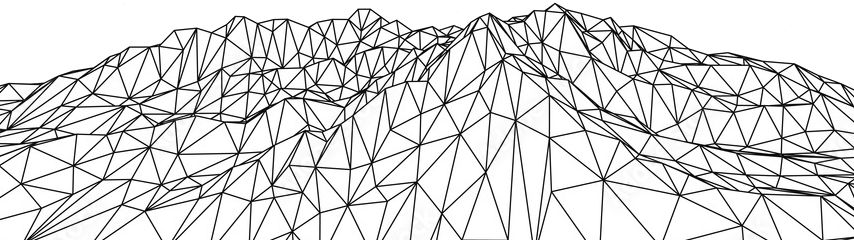
\includegraphics[width=\paperwidth]{../Unidad 2/Images/cover_bg}
\end{document}

\restoregeometry
\addtocontents{toc}{\setcounter{tocdepth}{3}}
\tableofcontents
\newpage
\chapter{}
\pagestyle{fancy}
\newpage
\thispagestyle{plain}
\section{Fracciones y decimales}
\subsection{Equivalencias de fracciones y decimales}
\subsection{Decimales peri\'odicos}
\subsubsection{Redondeo y truncamiento}

\newpage \thispagestyle{plain}

\section{Recta Num\'erica, Densidad y Orden}
\subsection{Fracciones en la Recta Num\'erica, Densidad y Orden}
\subsection{Decimales en la Recta Num\'erica, Densidad y Orden}
\subsection{Orden de fracciones y decimales}
\subsubsection{Orden en los n\'umeros fraccionarios}
\subsubsection{Orden en los n\'umeros decimales}


\newpage \thispagestyle{plain}
\section{Problemas con sumas y restas}
\subsection{N\'umeros con signo, recta y orden}
\subsection{Suma y resta de n\'umeros con signo}
\subsubsection{Suma de numeros con signo}
\subsubsection{Conmutatividad aditiva}
\subsubsection{Resta de n\'umeros con signo}
\newpage \thispagestyle{plain}
\section{Multiplicaci\'on con n\'umeros fraccionarios y decimales}
\subsection{Multiplicaci\'on con n\'umeros fraccionarios}
\subsection{Multiplicaci\'on con n\'umeros decimales}
\newpage \thispagestyle{plain}
\section{Divisi\'on con n\'umeros fraccionarios y decimales}
\newpage \thispagestyle{plain}
\section{\'Angulos, tri\'angulos y cuadril\'ateros}
\subsection{\'Angulos y rectas paralelas}
\subsection{Suma de los \'angulos interiores de un tri\'angulo y de un cuadril\'atero}
\subsubsection{\'Angulos de un tri\'angulo}
\subsubsection{\'Angulos de un cuadril\'atero}
\newpage \thispagestyle{plain}
\section{Tri\'angulos, cuadril\'ateros y congruencia}
\subsection{Criterios de congruencia}

\newpage \thispagestyle{plain}
\chapter{}
\newpage \thispagestyle{plain}
\section{Jerarqu\'ia de operaciones y signos de agrupaci\'on}
\boxabstract{Aprendizajes esperados}{
  Determina y usa la jerarquía de operaciones y los paréntesis en operaciones con números naturales, enteros y
  decimales (para multiplicación y división, sólo números positivos).
}

\subsection{Jerarqu\'ia de operaciones y signos de agrupaci\'on}
Dentro de las operaciones básicas de la aritmética existe una \textbf{jerarquía de operaciones}, es decir un
\textbf{orden}.

Recuerda cuando estabas en primaria y empezabas a leer, ¿qué aprendiste primero? Seguro fueron las vocales,
después fueron sílabas, después palabras completas hasta poder llegar a los enunciados y dentro de los enunciados
vienen los signos de puntuación, las comas, los dos puntos, el punto y seguido, el punto aparte, etc.
Y entendiste la importancia de los signos de puntuación.

En los siguientes enunciados podemos observar ejemplos:
\begin{center}
  \begin{minipage}{0.4\textwidth}
    \begin{bA}
      Perdón imposible, castigarlo.\\
      Perdón, imposible castigarlo.
    \end{bA}
  \end{minipage}
\end{center}

Como podemos ver el significado de ambas expresiones son diferentes, bueno de eso se trata, en las matemáticas
existen reglas que si no se siguen el resultado de la operación sería incorrecto.

La operación de suma, resta, multiplicación y división tienen el siguiente orden:
\begin{figure}[H]
  \centering
  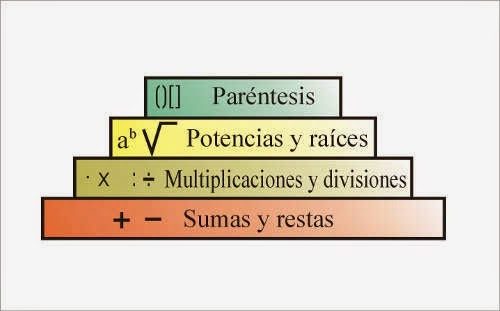
\includegraphics[width=0.5\textwidth]{./Unidad 2/Images/jerarquia.jpg}
\end{figure}

\subsubsection{Ejemplo 1: En este ejercicio haremos uso del paréntesis}

\[( 10 + 2 ) / 3 - 2\]

Observemos en este primer ejemplo se tiene un paréntesis y tiene mayor jerarquía, por lo que primero se realiza
esta operación.

\[12 / 3 - 2\]

Seguimos con el operador que tiene la jerarquía mas alta que es la división, y vamos de izquierda a derecha y
realizamos la operación.

\[4 - 2\]

Y por último, al resultado se le restan 2. Por lo que la operación nos queda:

\[( 10 + 2 ) / 3 - 2 = 2\]



\subsubsection{Ejemplo 2: En este ejercicio no utilizaremos el paréntesis}


Ahora vamos a ver el mismo problema pero sin el paréntesis.

\[5 + 6 / 2 - 2\]

Observemos que ahora la jerarquía mas alta la tiene primero la división, ya que no existe ningún paréntesis.

\[8 + 2 - 2 = 8\]

Vamos de izquierda a derecha, hacemos primero la suma y luego la resta y tenemos el resultado, como podemos apreciar
la gran importancia de respetar el orden de las operaciones para poder encontrar el resultado correcto.


\subsubsection{Ejemplo 3: En este ejercicio explicaremos un poco más detallado}

\[4 - 6 / 2 + 5 \times 2\]

Vamos de izquierda a derecha y hacemos la división por que en este ejemplo es el operador con mas jerarquía.

\[4 - 3 + 5 \times 2\]

Luego vamos de izquierda a derecha buscando el operador que tiene la mayor jerarquía para hacer la operaci\'on.
El cual es la multiplicaciónn.

\[4 - 3 + 10\]

Seguimos con la resta por izquierda y luego por la derecha

\[1 + 10\]

Por ultimo el resultado es el número 11.

\[4 - 6 / 2 + 5 \times 2 = 11\]

\newpage


\begin{problemas}

\end{problemas}

\newpage \thispagestyle{plain}
\section{Resolución de problemas con valores faltantes}
\boxabstract{Aprendizajes esperados}{Calcula valores faltantes en problemas de proporcionalidad directa,
  con constante natural, fracción o decimal (incluyendo tablas de variación).}

\subsection{Proporcionalidad directa y valor faltante}
\begin{boxK}
  \begin{center}\textbf{Inicio}\end{center}
  Menhir el arquitecto hizo un obelisco para conmemorar los setenta y seis años de su padre.
  Ahora hace un obelisco de menor tamaño, pero con la misma forma y del mismo material
  que el de su padre, para celebrar el decimonoveno cumpleaños de su hijo.
  \begin{enumerate}
    \item Las medidas de los obeliscos de Menhir están en la misma proporción que hay entre las
          edades de su padre y de su hijo. Si la altura del obelisco hecho en honor al padre es de
          12.2 m, ¿qué altura tiene el obelisco dedicado al hijo?

    \item Los obeliscos tienen base cuadrada. Si la base del obelisco dedicado al hijo tiene una
          longitud de 0.80 m por lado, ¿cuánto mide el lado de la base del obelisco más grande?
    \item Compartan sus respuestas y procedimientos con sus compañeros y escriban en su cuaderno
          el procedimiento que les parezca más acertado.
  \end{enumerate}
\end{boxK}

\begin{enumerate}
  \item En el local de jugos de Ana para preparar dos litros de agua de frutas se agregan,
        además de las frutas, cinco cucharadas de azúcar. Contesta lo siguiente
        \begin{enumerate}
          \item Si se mantiene la misma proporción, ¿cuántas cucharadas se necesitan para preparar ocho litros?
          \item Si agregó 33 cucharadas, ¿cuántos litros preparó?
          \item Si Ana utilizó 15 cucharadas, ¿cuántos litros prepararó?
          \item ¿Cuántas cucharadas se requieren para preparar un litro de agua?
        \end{enumerate}
  \item  Para llenar un vitrolero se necesitan cuatro litros de agua. Completa la tabla para
        saber cuántas cucharadas necesita Ana.
        \begin{figure}[H]
          \centering
          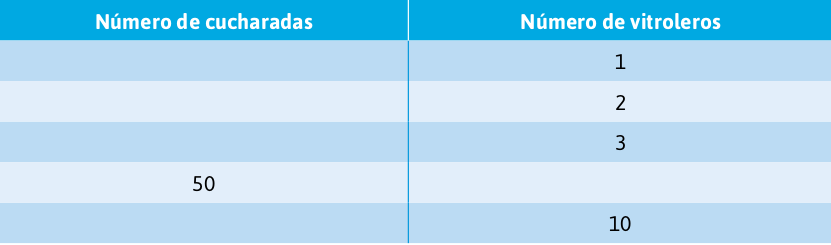
\includegraphics[width=0.6\linewidth]{tabla_vitrolero.png}
          \captionof{table}{}
          \label{tab:tabla_vitrolero}
        \end{figure}
        \begin{enumerate}
          \item ¿Cuántas cucharadas se necesitan para preparar un vitrolero?
          \item Si el número de vitroleros aumenta al doble, ¿cómo se incrementa el número de
                cucharadas? ¿Y si aumenta al triple?
          \item Explica en tu cuaderno, cómo determinarías el número de cucharadas a partir del
                número de vitroleros.
        \end{enumerate}

  \item Durante el Renacimiento, el estudio de la anatomía humana tuvo gran auge. Uno
        de los trabajos más conocidos es \emph{El hombre de Vitrubio} (ver figura \ref{fig:Hombre-de-Vitruvio}) de Leonardo
        da Vinci. Una de las proporciones más interesantes en esta obra es la relación entre
        la estatura de la figura y la distancia entre el ombligo y la base de los pies.

        \begin{minipage}{0.45\textwidth}
          \begin{figure}[H]
            \centering
            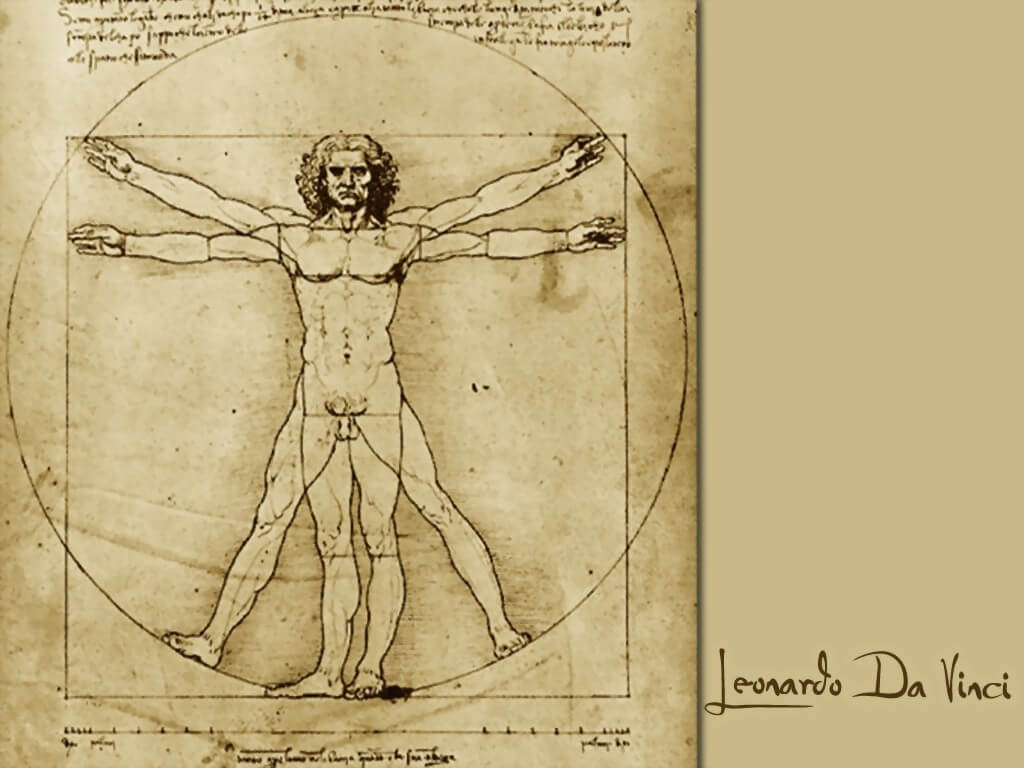
\includegraphics[width=\linewidth]{Hombre-de-Vitruvio.jpg}
            \captionof{figure}{Obra de Leonardo Da Vinci, titulada \emph{El hombre de Vitrubio}}
            \label{fig:Hombre-de-Vitruvio}
          \end{figure}
        \end{minipage}\hfill
        \begin{minipage}{0.45\textwidth}
          \begin{boxH}
            Dos magnitudes tienen una relación de proporcionalidad directa si al aumentar o
            disminuir una la otra aumenta o disminuye, respectivamente, en la misma proporción.
            En este caso, al calcular la razón entre un valor de la primera magnitud y su correspondiente
            de la otra magnitud, siempre obtendremos un número constante.
            Si en una relación de proporcionalidad directa se desconoce un valor, se dice que
            se trata de un problema de valor faltante.
          \end{boxH}
        \end{minipage}

        \begin{boxE}
          En \emph{El hombre de Vitrubio} se dice que la razón de su estatura respecto a la distancia
          del ombligo a los pies es perfecta y su valor es un número decimal no periódico e
          infinito: 1.61803\dots llamado \emph{proporción aúrea} (que redondeamos a 1.62).
        \end{boxE}

        \begin{enumerate}
          \begin{figure}[H]
            \centering
            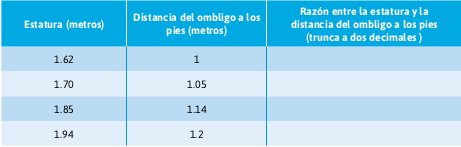
\includegraphics[width=0.6\linewidth]{tabla_hombre.png}
          \end{figure}
          \item Completa la tabla que relaciona la estatura de cuatro personas y la distancia de
                su ombligo a sus pies.
          \item ¿Qué observas en la última columna?

        \end{enumerate}

  \item Contesta lo siguiente.
        \begin{enumerate}
          \item ¿Cuál es la estatura de Carlos si la distancia de su ombligo al piso es de 1.10 m?
          \item Si la estatura de María es 1.49 m, ¿Cuál es la distancia de su ombligo al piso?
          \item ¿Qué operaciones hicieron para resolver estos problemas?
        \end{enumerate}
\end{enumerate}

\begin{boxH}
  Si la razón entre dos datos correpondientes de dos conjuntos es siempre la misma,
  se dice que ese valor es una \textbf{constante de proporcionalidad}. En una relación de
  proporcionalidad directa al multiplicar los datos del segundo conjunto por la constante
  de proporcionalidad se obtienen los datos correspondientes del primer conjunto, y
  viceversa, multiplicando por el \textbf{\color{cyan}inverso multiplicativo} de esa constante.
\end{boxH}

\begin{boxH}
  \textbf{\color{cyan}Inverso multiplicativo.}
  El inverso multiplicativo de un número es aquel que al
  multiplicarlo por el primero da como resultado 1.
  Así, el inverso de 5 es $\dfrac{1}{5}$, porque $5\cdot \dfrac{1}{5}=1$
\end{boxH}

\begin{boxK}
  \begin{center}\textbf{Cierre}\end{center}
  Regresa al problema inicial, identifica una relación de proporcionalidad directa y calcula
  la constante de proporcionalidad.
  Revisa tus respuestas a los incisos $a$ y $b$ y valida el procedimiento del inciso $c$.
\end{boxK}
\newpage
\subsection{Proporcionalidad y valor unitario}

\begin{boxK}
  \begin{center}\textbf{Inicio}\end{center}
  Manolo y Sebastián compraron una bolsa con 100 canicas como la que se muestra en la
  figura, por \$80.00. Manolo aportó \$32.00 y Sebastián completó el pago.
  \begin{enumerate}
    \item ¿Cuánto pagó Sebastián?
    \item ¿Te parece justo que, al repartirlas, cada uno tenga 50 canicas? ¿Por qué?
    \item ¿Cuántas canicas debería recibir cada uno de acuerdo con lo que aportaron?
    \item Explica cómo decidiste repartir las canicas entre Manolo y Sebastián, y por qué
          consideras que de esa manera el reparto es justo.
  \end{enumerate}
\end{boxK}

\begin{enumerate}
  \begin{minipage}[t]{0.3\textwidth}
    \begin{figure}[H]
      \centering
      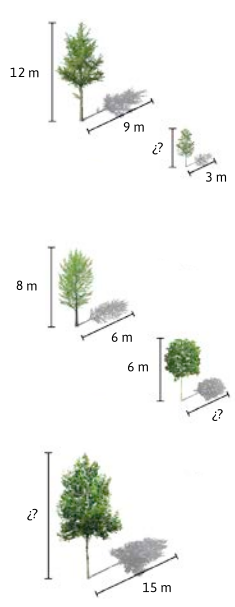
\includegraphics[width=\linewidth]{fig_sombras.png}
      \captionof{figure}{}
      \label{fig:fig_sombras}
    \end{figure}
  \end{minipage}\hfill
  \begin{minipage}[t]{0.65\textwidth}
    \item En un día soleado los objetos forman sombras y, a la misma hora, la altura y la
    sombra de diferentes objetos es proporcional.
    \begin{flushright}
      \begin{figure}[H]
        \centering
        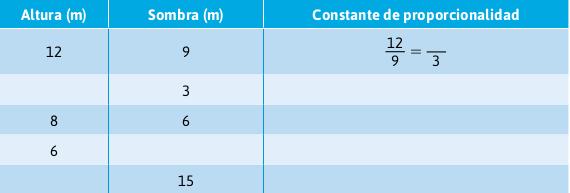
\includegraphics[width=0.85\linewidth]{tabla_sombras.png}
        \captionof{table}{}
        \label{tab:tabla_sombras}
      \end{figure}
    \end{flushright}
    \begin{enumerate}
      \item Con la información de la figura completa la tabla \ref{tab:tabla_sombras}.
      \item ¿Cómo son los números de la última columna?
      \item Si la sombra de un árbol mide 7.5 m, ¿cómo calcularías su altura? Explica.
      \item En primaria aprendiste a ubicar puntos en el plano cartesiano por medio de
            coordenadas. Ubica los puntos cuyas coordenadas corresponden a la altura y sombra de los árboles
      \item La gráfica representa la relación entre la sombra y la altura de un árbol. Unan los
            puntos que marcaron. ¿Qué observan?
    \end{enumerate}
  \end{minipage}

  \begin{figure}[H]
    \centering
    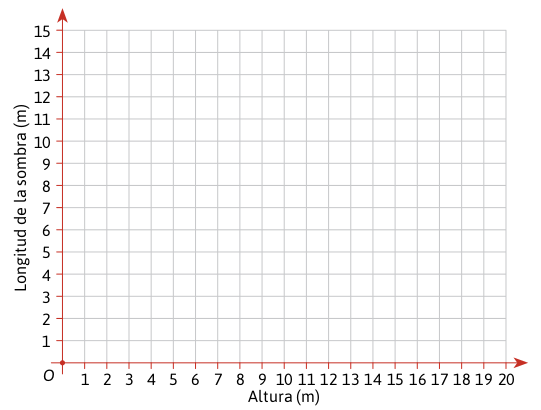
\includegraphics[width=.7\linewidth]{plano_sombras.png}
  \end{figure}

  \begin{figure}[H]
    \centering
    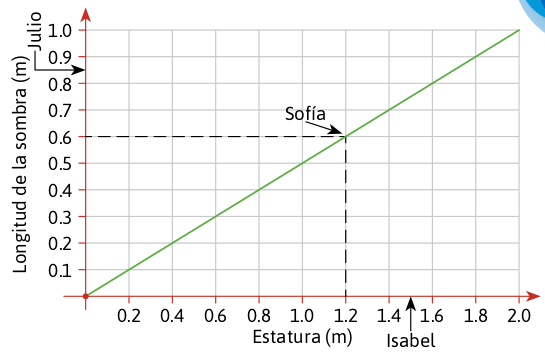
\includegraphics[width=0.6\linewidth]{graficas_sombras.png}
    \captionof{figure}{}
    \label{fig:graficas_sombras}
  \end{figure}

  \item La gráfica representa la relación entre la estatura de
        Sofía, Isabel y Julio y sus correspondientes sombras
        a las cuatro de la tarde de un día soleado. Obsérvenla y contesten.
        \begin{enumerate}
          \item Sofía mide 1.20 m y su sombra, 0.60 m. Si la estatura
                de Isabel es 1.50 m, ¿cuánto mide la longitud de su sombra?
          \item La sombra de Julio tiene una longitud de 0.85 m. ¿Cuál es su estatura?
          \item Si Efrén, un amigo de Sofía, mide 1.84 m, ¿cuánto mediría su sombra?
          \item ¿Cuánto vale la constante de proporcionalidad entre la estatura de las personas y la longitud de su sombra?
          \item ¿Cuánto mide la sombra de un objeto cuya altura es de 1 m?
          \item Compara los resultados con los de tus compañeros y juntos describan cómo usar
                la gráfica para obtener uno de los datos a partir del otro.
        \end{enumerate}

        \begin{boxH}
          Si dos o más razones tienen el mismo valor, entonces son \textbf{proporcionales}. El valor
          de esa razón corresponde a la \textbf{constante de proporcionalidad}.
        \end{boxH}

  \item Marca en la casilla las razones que forman una proporción.\\

        \begin{hoptboxes}
          \item $\dfrac{3}{4}   \text{ y } \dfrac{21}{28}$
          \item $\dfrac{32}{5}  \text{ y } \dfrac{96}{15}$
          \item $\dfrac{33}{42} \text{ y } \dfrac{17}{21}$
          \item $\dfrac{4}{5}   \text{ y } \dfrac{9}{12}$
          \item $\dfrac{1}{11}  \text{ y } \dfrac{3}{30}$
        \end{hoptboxes}

  \item La distancia que recorre un automóvil es proporcional al consumo de gasolina.
        Un automóvil recorre 180 km y gasta 12 L de gasolina.
        \begin{enumerate}
          \item ¿Cuántos kilómetros recorre con un litro?
          \item ¿Cuántos litros necesita para recorrer 480 km?
          \item ¿Cuál es el valor, en kilómetros, de la constante de proporcionalidad de la
                distancia recorrida, por cada litro de gasolina consumido?
        \end{enumerate}
        \begin{boxH}
          En una relación de proporcionalidad el valor unitario es el valor de una de las
          magnitudes cuando el de la magnitud correspondiente es igual a 1; por ejemplo, los
          kilómetros que recorre un automóvil con 1 L de gasolina o el precio de un libro. El
          valor unitario es numéricamente igual a la constante de proporcionalidad.
        \end{boxH}
\end{enumerate}

\begin{boxK}
  \begin{center}\textbf{Cierre}\end{center}

  \begin{enumerate}
    \item A partir de lo que aprendiste en esta lección resuelve nuevamente el problema
          inicial. Verifica tus respuestas previas y compara tus procedimientos anteriores
          con los que aprendiste. ¿Ambos fueron correctos? ¿Cuál te parece más
          adecuado? ¿Por qué?
    \item Un tubo de 2 m de longitud pesa 16 kg. ¿Cuál será el peso de un tubo del mismo
          tipo, pero con 3 m de longitud?
  \end{enumerate}
\end{boxK}

\newpage

\subsection{Resolución de problemas de proporcionalidad directa}
\begin{boxK}
  \begin{center}\textbf{Inicio}\end{center}
  A Sofía y Pablo les tomaron una fotografía al lado de un árbol. Sofía sabe que su estatura es
  de 1.20 m y al medir con una regla su altura en la foto obtuvo 4 cm.
  \begin{enumerate}
    \item ¿Cómo obtendrías la estatura real de Pablo y la altura del árbol con base en la
          foto?
    \item Si en la fotografía el árbol mide 10 cm, ¿cuál es su altura?
    \item Si la altura real de Pablo es de 1.50 m, ¿cuánto mide su imagen en la fotografía?
    \item Escribe en tu cuaderno el procedimiento que seguiste.
    \item Compara tus resultados y procedimientos con los de tus compañeros. Argumenten la validez de los mis
  \end{enumerate}

\end{boxK}

\begin{enumerate}
  \item Las medidas de una plaqueta electrónica para teclado son de 32 cm por 24 cm. Si
        en una computadora se instalara una plaqueta, sin reducirla, el teclado mediría
        112 cm por 336 cm en vez de 14 cm por 42 cm que es lo usual.
        \begin{enumerate}
          \item ¿De qué tamaño deberán ser las plaquetas electrónicas para un teclado de tamaño común?
          \item ¿Cuánto se debe reducir la plaqueta grande para que sea del tamaño de una usual?
          \item Explica cómo obtuviste la respuesta, compara tu método con el de un compañero
                y expongan al resto del grupo el método que les parezca más adecuado.
        \end{enumerate}

  \item La junta directiva de la secundaria Lázaro Cárdenas decidió que en las bibliotecas
        de aula haya 3 libros por cada cuatro alumnos.
        \begin{enumerate}
          \item Si en el salón de Edna hay 44 alumnos, ¿cuántos libros debe haber?
          \item Explica cómo determinaste el número de libros.
          \item Completa la siguiente tabla.
                \begin{figure}[H]
                  \centering
                  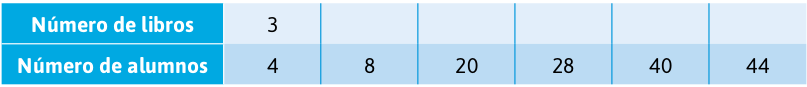
\includegraphics[width=0.6\linewidth]{tablaLibrosAlumnos.png}
                  \captionof{figure}{}
                  \label{fig:tablaLibrosAlumnos}
                \end{figure}
          \item Escribe la constante de proporcionalidad que relacione el número de libros y el
                número de alumnos.
        \end{enumerate}
  \item  Una tortuga avanza 48 cm en 12 segundos.
        \begin{enumerate}
          \item ¿Qué distancia recorrerá en un minuto si camina con la misma rapidez?
          \item Completa la siguiente tabla que Eduardo hizo para resolver el problem
                \begin{figure}[H]
                  \centering
                  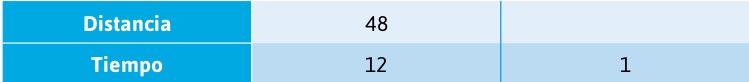
\includegraphics[width=0.6\linewidth]{tablaDistanciaTiempo.png}
                  \captionof{figure}{}
                  \label{fig:tablaDistanciaTiempo}
                \end{figure}
          \item Eduardo escribió 4 en la casilla vacía, pero considera que está mal porque no es
                posible que la tortuga en 1 min recorra menos distancia que en 12 s. ¿En qué
                consiste su error?
          \item En tu cuaderno elabora una tabla como la de Eduardo, en el reglón de tiempo
                incluye: una hora, un día y una semana. Escribe las distancias correspondientes
                y comparte tus respuestas con el resto del grupo. Retoma la pregunta anterior y
                explica en qué consistió el error de Eduardo.
        \end{enumerate}


  \item Si 4 toronjas se venden en 25 pesos, ¿cuánto cuestan 6 toronjas?
        \begin{enumerate}
          \item Completa la tabla con el valor que falta (valor faltante).
                \begin{figure}[H]
                  \centering
                  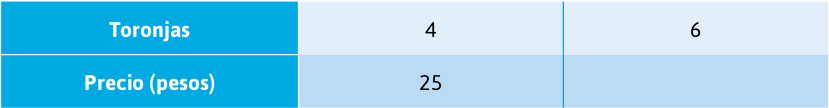
\includegraphics[width=0.6\linewidth]{tabla_toronjas.png}
                  \captionof{table}{}
                  \label{tab:tabla_toronjas}
                \end{figure}
          \item Explica cómo obtuviste la respuesta.
          \item Completa la proporción a partir de los datos del problema y calcula el valor faltante.
                \[\dfrac{25}{4} = \dfrac{}{6}\]
          \item ¿El valor faltante que propusiste en la tabla valida la igualdad anterior? Explica.
        \end{enumerate}
  \item Sofía leyó 25 páginas de un libro en 40 min. ¿Cuántas páginas leerá en 80 min si continua leyendo al mismo ritmo?
        \begin{enumerate}
          \item Escribe una proporción con un valor faltante para determinar cuántas páginas leerá en 65 minutos.
                \[\dfrac{\text{ }}{\text{ }} = \dfrac{\text{ }}{\text{ }}\]
          \item Encuentra el valor faltante de la proporción anterior y verifica que se conserva la
                igualdad de las razones.
          \item ¿Cuánto se consume la vela cada minuto?
          \item ¿En cuánto tiempo se consume 1 cm de vela?
          \item Completa la tabla.
                \begin{figure}[H]
                  \centering
                  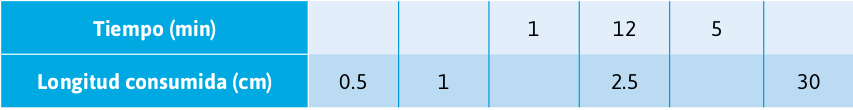
\includegraphics[width=0.6\linewidth]{tabla_longitud.png}
                  \captionof{table}{}
                  \label{tab:tabla_longitud}
                \end{figure}
        \end{enumerate}

  \item Un avión Boeing 747 mide 77 m de largo por 63 de ancho (esta medida
        indica la longitud de las alas de un extremo al otro). Un modelo a escala
        mide 44 cm de largo.
        \begin{enumerate}
          \item ¿Cuál es el ancho del modelo a escala?
          \item Explica tu procedimiento para resolver el problema.
          \item ¿Cuánto debe medir la altura de una ventana en el modelo a escala si en el avión
                real es de 0.7 m?
          \item ¿Cuál es la constante de proporcionalidad del modelo real al modelo a escala?
                En este caso la constante recibe el nombre de \emph{escala del modelo}.
        \end{enumerate}

  \item Una receta para hacer dulce de membrillo indica que la cantidad de fruta debe
        ser una vez y media la cantidad de azúcar. Contesta.
        \begin{enumerate}
          \item Si se usan 2 kg de membrillo, ¿cuántos kilogramos de azúcar se necesitan?
          \item ¿Y si se usan 5 kg de membrillo?
          \item Completa la tabla e indica la constante de proporcionalidad que relaciona la cantidad
                de membrillo y la cantidad de azúcar.
                \begin{figure}[H]
                  \centering
                  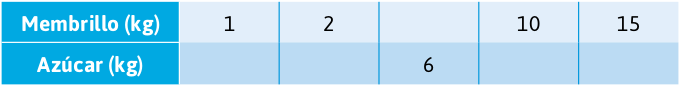
\includegraphics[width=0.6\linewidth]{tabla_azucar.png}
                  \captionof{table}{}
                  \label{tab:tabla_azucar}
                \end{figure}
          \item Si la cantidad de membrillo aumenta ocho veces, ¿cuánto aumentará la cantidad
                de azúcar?
          \item Si la cantidad de membrillo disminuye a la mitad, ¿cómo cambiará la cantidad de
                azúcar?
        \end{enumerate}
  \item Un tren tarda 40 min en recorrer 130 km. ¿Cuánto tardará en recorrer 195 km si
        mantiene la misma rapidez? Explica tu procedimiento.
  \item Al medir el ritmo cardiaco de un paciente, durante 5 s el médico le dijo: \emph{su
          pulso está bien, usted tiene 72 pulsaciones por minuto}.
        \begin{enumerate}
          \item ¿Qué cálculo piensas que hizo el médico para saber el número de pulsaciones
                por minuto si sólo tomó el pulso por 5 segundos?
        \end{enumerate}
  \item Para hacer mermelada de fresa se necesitan 3 kg de fresas frescas por cada 2 kg
        de azúcar. Karol sólo tiene 2.5 kg de fresas. Contesta.
        \begin{enumerate}
          \item ¿Cuánta azúcar debe utilizar para que el sabor de la mermelada sea el mismo que
                el de la receta original?
          \item Explica el procedimiento que seguiste para resolver el problema.
          \item Si Antonio tiene 3.6 kg de azúcar, ¿cuántos kilogramos de fresas necesita si quiere emplear toda la azúcar?
          \item Explica tu procedimiento para resolver el problema.
          \item Alejandro cuenta con $\dfrac{3}{4}$ kg de fresas. ¿Cuántos kilogramos de azúcar debe emplear?
        \end{enumerate}
  \item Una bomba mueve 300 L de agua por hora. ¿Cuánto tardará en llenar un depósito de 3 200 litros?
  \item Una compañía envasadora necesita comprar una máquina que lave al menos 900
        botellas en 1 hora.
        \begin{enumerate}
          \item El vendedor les muestra una máquina que lava 60 botellas en 5 min. ¿Esta máquina cumple con los requerimientos de la compañía? ¿Por qué?
          \item El instructivo de otra máquina muestra la gráfica de
                la figura \ref{fig:tabla_instructivo}. ¿Esta máquina cumple las necesidades de la compañía? ¿Por qué?

          \item ¿Cuál de las dos máquinas lava más botellas por unidad de tiempo?
                \begin{figure}[H]
                  \centering
                  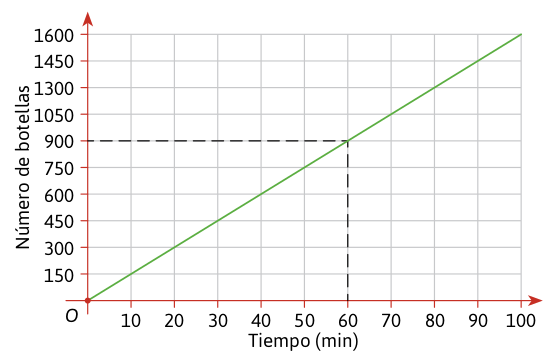
\includegraphics[width=0.5\linewidth]{tabla_instructivo.png}
                  \captionof{figure}{}
                  \label{fig:tabla_instructivo}
                \end{figure}

        \end{enumerate}
\end{enumerate}

\begin{boxK}
  \begin{center}\textbf{Cierre}\end{center}

  \begin{enumerate}
    \item Retoma el problema de la sección Inicio y verifica tus respuestas.
          \begin{enumerate}
            \item ¿Cuál es la constante de proporcionalidad que relaciona las medidas de los
                  objetos reales con los de la fotografía?
          \end{enumerate}
    \item ¿Cómo verificarías sin dividir la proporción $\dfrac{7.5}{1.5} = \dfrac{15}{3}$?
    \item Encuentra el valor faltante en las siguientes proporciones.\\

          \begin{hoptions}
            \item $\dfrac{}{25} = \dfrac{32}{8} $
            \item $\dfrac{25}{25} = \dfrac{}{10}$
            \item $\dfrac{30}{} = \dfrac{54}{9} $
          \end{hoptions}
  \end{enumerate}
\end{boxK}

\begin{boxH}
  ¿El perímetro de un cuadrado es proporcional a las medidas de sus lados?
  Explica.\\
  Si las medidas de un rectángulo se duplican, ¿el área del nuevo rectángulo
  también se duplica respecto al inicial? Justifica tu respuesta.
\end{boxH}

\newpage \thispagestyle{plain}
\section{Porcentajes}

\boxabstract{Aprendizajes esperados}{Resuelve problemas de cálculo de porcentajes, de tanto por ciento y de la cantidad base.}

\subsection{Tanto por ciento}

\begin{boxK}
  \begin{center}\textbf{Inicio}\end{center}
  \begin{enumerate}
    \item El grupo 1º C ha organizado una competencia para elegir al equipo que los
          representará en el torneo de tiros libres de basquetbol de la escuela. Cada
          equipo está formado por cuatro alumnos y cada uno debe realizar un número distinto
          de lanzamientos a la canasta: uno debe hacer 20, otro 10, otro 5 y
          otro 4. Ganará el equipo que enceste más veces.
          En un equipo están Pablo, Sofía, Alfonso y Nayhelli, quienes en los entrenamientos
          tuvieron el desempeño que muestra la tabla.
          \begin{figure}[H]
            \centering
            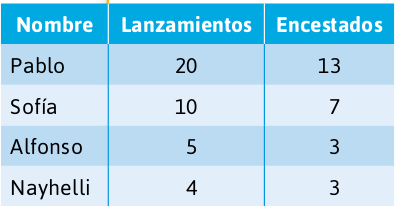
\includegraphics[width=0.4\linewidth]{tabla_lanzamientos.png}
            \captionof{figure}{}
            \label{fig:tabla_lanzamientos}
          \end{figure}
          \begin{enumerate}
            \item ¿Quién es el mejor encestador? ¿Cómo lo sabes?
            \item ¿Cuántos lanzamientos le asignarías a cada uno para obtener el mejor resultado en la competencia?
            \item Compara tus respuestas con las de tus compañeros. Respecto a
                  esos cuatro alumnos, ¿cómo decidieron quién es el mejor y el
                  peor encestador? ¿Con qué criterios asignaron el número de
                  lanzamientos a cada uno? Argumenten sus respuestas.
          \end{enumerate}

  \end{enumerate}
\end{boxK}

\begin{enumerate}
  \item En la Academia de Policía evaluaron la condición física de los cadetes.
        \begin{enumerate}
          \item Marca las afirmaciones equivalentes.\\
                \begin{hoptboxes}
                  \item Tres quintas partes tuvo excelentes resultados.\\
                  \item Veinte de cada veinticinco cadetes tuvieron excelentes resultados.\\
                  \item De cada cinco alumnos, cuatro lograron excelentes resultados.\\
                  \item De cien cadetes, ochenta tuvieron excelentes resultados.\\
                  \item Ocho de cada diez lograron excelentes resultados.\\
                \end{hoptboxes}
          \item Compara tus respuestas con las de tus compañeros y explíquenlas.
          \item Expresa en cada caso el número de cadetes con buenos resultados como una fracción
                con denominador 100. ¿Qué observas?
        \end{enumerate}

        \begin{boxH}
          Por ciento significa \emph{por cada cien} y se refiere a la razón entre una cantidad dada
          y un total de 100 elementos; también se llama tanto por ciento, esto es, \emph{una cantidad por cada cien}.
          Se usa el símbolo \% para indicar un tanto por ciento: 27 de
          cada 100 se expresa como 27 o 27\%.
        \end{boxH}

  \item Completa la tabla \ref{fig:tabla_tantoporciento}.

        \begin{figure}[H]
          \centering
          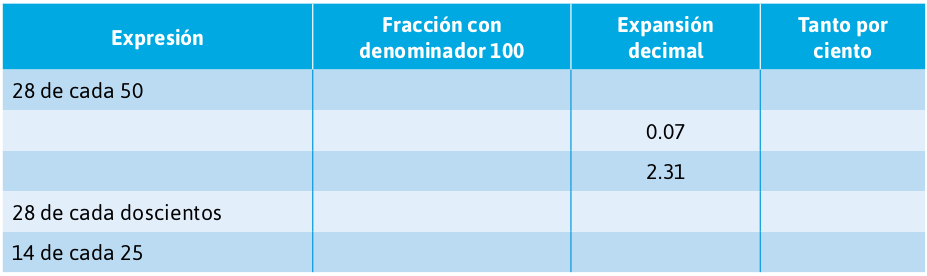
\includegraphics[width=0.7\linewidth]{tabla_tantoporciento.png}
          \captionof{figure}{}
          \label{fig:tabla_tantoporciento}
        \end{figure}

        \begin{enumerate}
          \item En su cuaderno escriban qué relación hay entre la expansión decimal y el tanto por
                ciento.
        \end{enumerate}
  \item Escribe el tanto por ciento que representa la parte sombreada de las
        figuras o coloreen el porcentaje que corresponde.
        \begin{figure}[H]
          \centering
          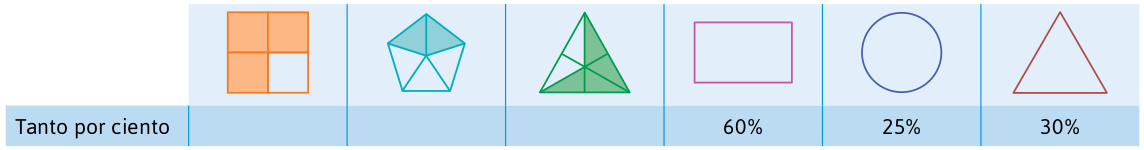
\includegraphics[width=0.8\linewidth]{tabla_figuras.png}
          \captionof{figure}{}
          \label{fig:tabla_figuras}
        \end{figure}
        \begin{boxH}
          Para convertir un decimal en tanto por ciento, se multiplica el decimal por 100 y
          se agrega el signo \%.
        \end{boxH}
\end{enumerate}

\begin{boxK}
  \begin{center}\textbf{Cierre}\end{center}

  \begin{enumerate}
    \item Retoma la actividad de la situación inicial y determina el porcentaje de encestes
          con respecto a los lanzamientos de cada alumno.
          \begin{enumerate}
            \item Resuelve nuevamente el inciso b. Explica cómo llegaste a esa conclusión.
            \item ¿Tus resultados iniciales fueron correctos? Justifica tus respuestas.
          \end{enumerate}
    \item El promedio de bateo se determina como la razón del número de hits que logra
          un jugador de beisbol entre la cantidad de turnos al bat.\\
          \begin{enumerate}
            \item  El legendario jugador de beisbol Babe Ruth de los Yanquis de Nueva York tuvo
                  un promedio de bateo de 0.34. ¿Qué significa ese número en porcentaje?
            \item Adrián \emph{el titán} González, bateador mexicano de los Dodgers de Los Ángeles,
                  tiene promedio de bateo de 0.29. ¿Quién es mejor bateador? Explica.
          \end{enumerate}
  \end{enumerate}
\end{boxK}
\newpage
\subsection{Cálculo del porcentaje}

\begin{boxK}
  \begin{center}\textbf{Inicio}\end{center}

  \begin{enumerate}
    \item Observa los anuncios.
          \begin{figure}[H]
            \centering
            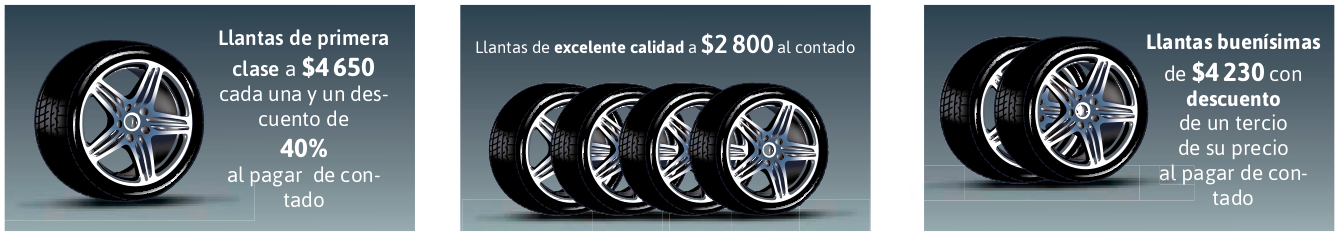
\includegraphics[width=\linewidth]{llantas.png}
            % \captionof{figure}{}
            % \label{fig:llantas}
          \end{figure}
          \begin{enumerate}
            \item Cuál es la mejor oferta si todas las llantas son del mismo tipo y marca?
            \item Compara tu respuesta con la de tus compañeros y argumenten por qué su elección es la mejor.
          \end{enumerate}
  \end{enumerate}
\end{boxK}
\begin{enumerate}
  \item Observa la nota del consumo del restaurante de la figura \ref{fig:nota_consumo} y
        contesten.

        \begin{minipage}[t]{0.2\textwidth}
          \begin{figure}[H]
            \centering
            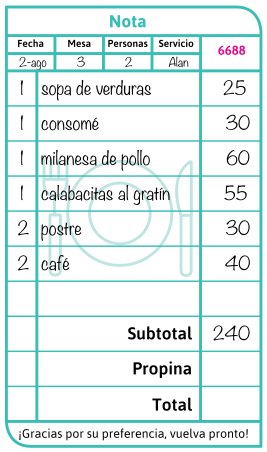
\includegraphics[width=\linewidth]{nota_consumo.png}
            \captionof{figure}{}
            \label{fig:nota_consumo}
          \end{figure}
        \end{minipage}\hfill
        \begin{minipage}[t]{0.75\textwidth}
          \begin{enumerate}
            \item Como propina, los comensales quieren dejar 10\% del precio de su consumo. ¿Qué cantidad deben anotar en la nota?\\
            \item Y si la cuenta fuera de \$534.00, ¿cuánto sería de propina?\\
            \item Escriban un procedimiento para obtener el 10\% de una cantidad.\\
            \item Comparen sus procedimientos con los del grupo. ¿Son iguales o diferentes? ¿Todos son correctos? Argumenten sus respuestas y valídenlas en grupo.\\
          \end{enumerate}
        \end{minipage}

        \begin{boxH}
          Cuando a una cantidad se aplica el tanto por ciento se involucran tres
          datos: el tanto por ciento o \textbf{tasa}, la cantidad a la que se le aplica esa tasa
          (\textbf{cantidad base}) y el resultado (\textbf{porcentaje}).
        \end{boxH}
  \item Calcula los porcentajes.
        \begin{enumerate}
          \item Obten el 10\% de las siguientes cantidades.\\

                \begin{hoptions}
                  \item 25 \rule{20mm}{0.2mm}
                  \item 36.8 \rule{20mm}{0.2mm}
                  \item 2445.9 \rule{20mm}{0.2mm}
                  \item 66 \rule{20mm}{0.2mm}
                \end{hoptions}
          \item Obten el 5\%.\\

                \begin{hoptions}
                  \item 25 \rule{20mm}{0.2mm}
                  \item 36.8 \rule{20mm}{0.2mm}
                  \item 2445.9 \rule{20mm}{0.2mm}
                  \item 66 \rule{20mm}{0.2mm}
                \end{hoptions}
          \item Calcula el 20\%.\\

                \begin{hoptions}
                  \item 25 \rule{20mm}{0.2mm}
                  \item 36.8 \rule{20mm}{0.2mm}
                  \item 2445.9 \rule{20mm}{0.2mm}
                  \item 66 \rule{20mm}{0.2mm}
                \end{hoptions}
          \item ¿Qué procedimiento seguiste para obtener los resultados? Explícalo al resto del grupo y valídenlos.\\
          \item Explica cómo calcular mentalmente el 1\% de cualquier cantidad.\\
        \end{enumerate}
  \item Calcula el 1\% de las siguientes cantidades.\\

        \begin{hoptions}
          \item 115.1 \rule{20mm}{0.2mm}
          \item 780 \rule{20mm}{0.2mm}
          \item 300 \rule{20mm}{0.2mm}
          \item 66.6 \rule{20mm}{0.2mm}
        \end{hoptions}
  \item Calcula los porcentajes de las cantidades de la tabla \ref{fig:tabla_porciento}.\\

        \begin{figure}[H]
          \centering
          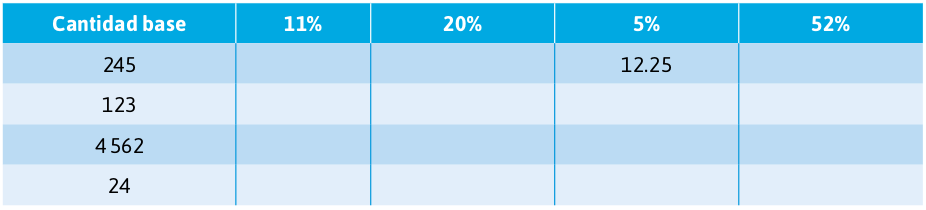
\includegraphics[width=.8\linewidth]{tabla_porciento.png}
          \captionof{figure}{}
          \label{fig:tabla_porciento}
        \end{figure}
  \item Realiza los siguientes ejercicios.
        \begin{enumerate}
          \item Calculen el 35\% de 240 pesos.
          \item Escriban 35\% como una fracción con denominador 100.
          \item Completen la siguiente proporción.
                \[\dfrac{35}{100} = \dfrac{}{240}\]
          \item Comparen su resultado con el inciso a. ¿Qué observan?
          \item Expliquen cómo calcular el porcentaje de una cantidad dada la tasa. Compartan
                sus propuestas en grupo y propongan ejercicios para aplicarlas. Verifiquen los
                resultados y utilícenlos como validación de sus procedimientos.
        \end{enumerate}
  \item Analiza la afirmación del recuadro.
        \begin{boxH}
          Para calcular el porcentaje de una cantidad basta multiplicar la cantidad base por
          la tasa y dividir entre 100.
        \end{boxH}
        \begin{enumerate}
          \item ¿Es correcta? ¿Por qué?
        \end{enumerate}
\end{enumerate}

\begin{boxK}
  \begin{center}\textbf{Cierre}\end{center}

  \begin{enumerate}
    \item Retoma la actividad de la situación inicial y según lo que aprendiste en la lección
          determina cuál es la oferta más económica. Observa que el hecho de
          anunciar un gran descuento no significa forzosamente un precio más barato.
    \item En una tienda anuncian un 20\% de descuento en todos sus productos. Observa
          la computadora.
          \begin{enumerate}
            \item ¿Cuál es su precio después de la rebaja? ¿Cómo obtuviste ese resultado?
            \item Calcula el 80\% del precio de la computadora y compara tu resultado con el del inciso a. ¿Qué observas?
            \item ¿Cómo calcularías el precio con descuento de una televisión que cuesta \$2 340.00? Indica su precio final.
            \item Compara tus resultados y procedimientos con los de tus compañeros y valídenlos con ayuda de su profesor.
          \end{enumerate}
  \end{enumerate}
\end{boxK}
\newpage
\subsection{Porcentajes y aplicaciones}
\begin{boxK}
  \begin{center}\textbf{Inicio}\end{center}

  \begin{enumerate}
    \item El entrenador de un equipo de beisbol debe comprar guantes y bates para todo el equipo.
          Revisa las ofertas de las tiendas El guante de oro y El bateador.
          \begin{figure}[H]
            \centering
            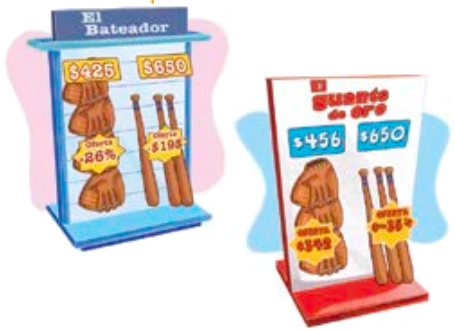
\includegraphics[width=.5\linewidth]{tiendas.png}
            \captionof{figure}{}
            \label{fig:tiendas}
          \end{figure}
          \begin{enumerate}
            \item ¿En qué tienda el guante tiene mayor descuento en pesos?
            \item ¿En cuál tiene mayor tasa de descuento?
            \item ¿En cuál tienda son más baratos los bates?
            \item ¿Cuáles bates tienen mayor tasa de descuento?
            \item ¿Dónde comprarías tres bates y nueve guantes?
            \item ¿Cuánto pagarías y cuánto ahorrarías?
            \item Compara tus resultados y tus procedimientos con los de tus
                  compañeros y argumenten por qué piensan que su elección
                  es correcta.
          \end{enumerate}
  \end{enumerate}
\end{boxK}

\begin{enumerate}
  \item La gráfica muestra la composición de una escuela de 2 400 personas.
        \begin{figure}[H]
          \centering
          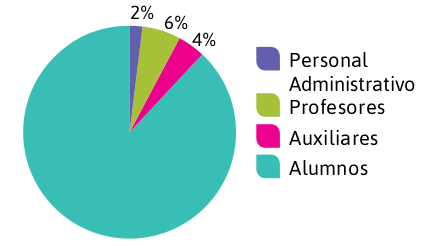
\includegraphics[width=.5\linewidth]{escuela_pie.png}
          \captionof{figure}{}
          \label{fig:escuela_pie}
        \end{figure}
        \begin{enumerate}
          \item ¿Cuántas personas trabajan en la administración?
          \item ¿Cuántos profesores hay en esa escuela?
          \item ¿Cuántas personas son auxiliares?
          \item ¿Cuál es el porcentaje de alumnos?
          \item ¿Cuántos alumnos tiene la escuela?
        \end{enumerate}
  \item Don Lupe es carpintero y comenta que el precio de la madera aumentó 8\%, por lo
        que piensa cobrar 8\% más en todos los muebles y objetos que fabrique.
        \begin{figure}[H]
          \centering
          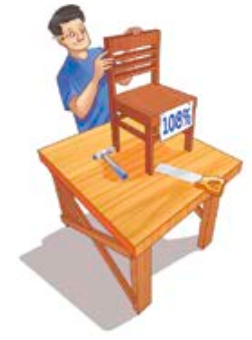
\includegraphics[width=.3\linewidth]{donLupe.png}
          \captionof{figure}{}
          \label{fig:donLupe}
        \end{figure}
        \begin{enumerate}
          \item Él considera que cobrando el 108\% del precio original de sus productos
                estaría cobrando el incremento que pretende. ¿Su razonamiento es correcto? Explica.
          \item ¿Cuál sería el nuevo precio de una silla que costaba \$250 pesos?
        \end{enumerate}
  \item En una tienda departamental Constanza compró el juego de sartenes que muestra
        el anuncio. El precio original era de \$348.00 y la cajera le comentó que sobre el
        precio final debía pagar el 16\% de IVA. Constanza sugirió pagar primero el IVA y
        después aplicar el descuento para, de esa manera, pagar menos.
        \begin{figure}[H]
          \centering
          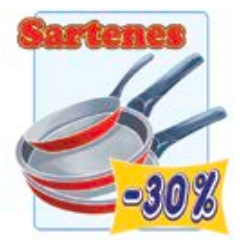
\includegraphics[width=.3\linewidth]{sartenes.png}
          \captionof{figure}{}
          \label{fig:sartenes}
        \end{figure}
        \begin{enumerate}
          \item ¿El razonamiento de Constanza es correcto? Explica.
          \item Compartan sus respuestas en grupo. ¿Creen que es mejor primero cobrar el IVA y
                luego hacer el descuento o al revés? ¿Por qué?
        \end{enumerate}
  \item Resuelve los siguientes problemas.
        \begin{enumerate}
          \item En la papelería La goma todos los precios incluyen IVA. Si el impuesto
                (16\%) que se paga por los colores es de \$4.00, ¿cuál es su precio sin IVA?
          \item En la misma papelería el papel para dibujo está en oferta. Si al precio,
                \$165.00, se le descuentan \$24.75, ¿de cuánto es la tasa de descuento?

          \item ¿Cómo obtuvieron el resultado de cada uno de los incisos anteriores? Expliquen
                sus procedimientos ante el grupo y entre todos propongan procedimientos para
                calcular la cantidad base dadas la tasa y el porcentaje, y para obtener la tasa,
                dadas la cantidad base y el porcentaje.
        \end{enumerate}
\end{enumerate}

\begin{boxK}
  \begin{center}\textbf{Cierre}\end{center}

  Retoma la actividad de la situación inicial y determina dónde es más conveniente
  comprar cada artículo deportivo. ¿Cuánto se ahorraría? ¿Coinciden tus
  respuestas con las que obtuviste al inicio? Valídalas con el resto del grupo
\end{boxK}

\begin{boxH}
  Como en la mercería \emph{El resguardo} están reetiquetando toda la mercancía, el gerente
  indica que el precio en la etiqueta debe incluir un descuento de 5\% y el 16\%
  del IVA . Una empleada piensa que basta con aumentar los precios un 11\%. ¿Su razonamiento
  es correcto? Justifica tu respuesta con ejemplos.
\end{boxH}



\newpage \thispagestyle{plain}
\section{Perímetros y áreas}
\boxabstract{Aprendizajes esperados}{Calcula el perímetro de polígonos y del círculo, y áreas de triángulos y cuadriláteros desarrollando
  y aplicando fórmulas.}

\subsection{Perímetro de polígonos}

\begin{boxK}
  \begin{center}\textbf{Inicio}\end{center}

  \begin{enumerate}
    \item Pablo necesita varios trozos de cordón para amarrar paquetes como el de la figura A y
          debe considerar, además, 80 cm para el moño.
          \begin{figure}[H]
            \centering
            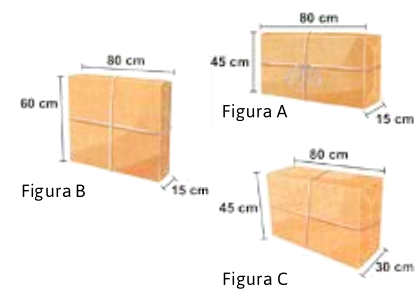
\includegraphics[width=.6\linewidth]{figuras_cajas.png}
            \captionof{figure}{}
            \label{fig:figuras_cajas}
          \end{figure}
          \begin{enumerate}
            \item ¿Qué cantidad de cordón ocupará Pablo?
            \item El paquete de la figura B es 15 cm más alto que el de la figura A. ¿Cuánto cordón más, del que ocupó en el primero, necesita Pablo para amarrarlo?
            \item El paquete de la figura C es 15 cm más ancho que el de la figura A. ¿Cuánto cordón más, del que ocupó en el primero, necesita para amarrarlo?
            \item En parejas justifiquen por qué el empaque de la figura C requiere más cordón que el de la figura B, aun cuando en ambos casos sólo una de las dimensiones se incrementa en 15 cm.
          \end{enumerate}
  \end{enumerate}
\end{boxK}

\subsubsection{Perímetro y expresiones algebraicas}

\begin{enumerate}
  \begin{minipage}[t]{.2\textwidth}
    \begin{figure}[H]
      \centering
      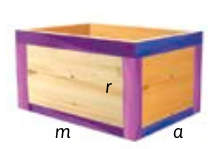
\includegraphics[width=\linewidth]{caja.png}
      \captionof{figure}{}
      \label{fig:caja}
    \end{figure}
  \end{minipage}\hfill
  \begin{minipage}[t]{.7\textwidth}
    \item Sofía compró una caja sin tapa como la de la figura \ref{fig:caja} para guardar fotografías,
    y quiere decorar las orillas de las caras con tiras de tela de colores: de color rosa
    a lo alto, moradas a lo largo y azules a lo ancho.

    \begin{enumerate}
      \item ¿Cuántas tiras de tela ocupará en cada cara de la caja?
      \item ¿Cuántas y de qué color serán las tiras de tela que ocupará?
    \end{enumerate}
  \end{minipage}

  \item Considera que la caja mide $r$ centímetros de alto, $m$ centímetros de largo
        y $a$ centímetros de ancho. Completa la tabla, expresa con esas letras el perímetro
        de una de las caras que se adornarán con las tiras indicadas.
        \begin{figure}[H]
          \centering
          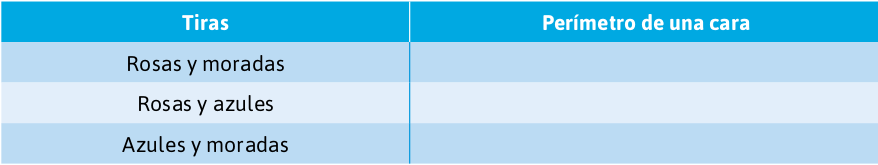
\includegraphics[width=.65\linewidth]{tabla_caja.png}
          \captionof{figure}{}
          \label{fig:tabla_caja}
        \end{figure}
        \begin{enumerate}
          \item Representen con las expresiones anteriores, el perímetro de todas las caras de la
                caja.
          \item ¿Cuántas tiras de cada color necesita Sofía para adornar toda la caja?
          \item En grupo compartan sus respuestas y validen cada una de ellas. Expresen con
                las letras $r$, $m$ y $a$ el total de tiras necesarias para adornar la caja.
        \end{enumerate}

        \begin{boxH}
          Una \textbf{expresión algebraica} es una combinación de literales (letras) para representar
          cantidades, y coeficientes (números) junto a ellas que indican cuántas veces se
          multiplica esa cantidad. La letra y el número forman un \textbf{término algebraico}.
        \end{boxH}

        \begin{boxH}
          Los términos algebraicos que tienen las mismas literales se conocen como \textbf{términos semejantes},
          y se simplifican sumando los coeficientes, por ejemplo, \[ 3a + 2a = 5a \].
        \end{boxH}

  \item Pedro, el hermano de Sofía, compró una caja de igual tamaño, y a partir de la idea de
        su hermana, optó por adornar con tiras de color azul, tanto el largo como el ancho de
        la caja y de verde los segmentos verticales.

        \begin{minipage}[t]{0.3\textwidth}
          \begin{figure}[H]
            \centering
            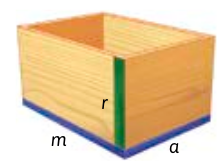
\includegraphics[width=\linewidth]{caja_sintapa.png}
            \captionof{figure}{}
            \label{fig:caja_sintapa}
          \end{figure}
        \end{minipage}\hfill
        \begin{minipage}[t]{0.7\textwidth}
          \begin{enumerate}
            \item Expresa algebraicamente la longitud total de la tira azul que se muestra en la figura \ref{fig:caja_sintapa}.
            \item Usa tu respuesta anterior para expresar algebraicamente el total de tela azul que
                  Pedro necesitará para decorar su caja.
            \item Expresa algebraicamente el total de tela (azul y verde) que Pedro utilizará para decorar su caja.
            \item Compara tu respuesta al inciso anterior con la que diste en el inciso (a de la actividad 2.
                  Escribe tus conclusiones en tu cuaderno.
            \item Si las cajas miden 12 cm de ancho, 20 cm de largo y 15 cm de alto, ¿cuánta tela ocuparán Sofía y Pedro?
          \end{enumerate}
        \end{minipage}


  \item Julián pintará en la pared una flecha, como la que aparece en la figura \ref{fig:flecha}.
        Para no rebasar los bordes colocará cinta adhesiva alrededor como se observa.

        \begin{minipage}[t]{0.3\textwidth}
          \begin{figure}[H]
            \centering
            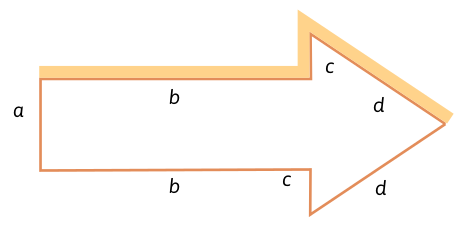
\includegraphics[width=\linewidth]{flecha.png}
            \captionof{figure}{}
            \label{fig:flecha}
          \end{figure}
        \end{minipage}\hfill
        \begin{minipage}[t]{0.7\textwidth}
          \begin{enumerate}
            \item En equipos expresen algebraicamente la cantidad de cinta adhesiva que ya colocó Julián.
            \item ¿Cuántas veces se debe colocar la cantidad $b + c + d$ de cinta alrededor de la flecha?
            \item Expresen algebraicamente el total de cinta que Julián colocará alrededor de la flecha.
            \item ¿Cuál es el perímetro de la figura \ref{fig:flecha}?
          \end{enumerate}
        \end{minipage}

        \begin{boxH}
          Una expresión algebraica cuyos términos tienen el mismo coeficiente es
          equivalente a un producto cuyos factores son el coeficiente y la expresión formada por
          las literales de la expresión original. Por ejemplo,
          \[ 2b + 2c + 2d = 2(b + c + d)\]
        \end{boxH}

        \begin{boxE}
          En las expresiones algebraicas, por simplicidad, para indicar un producto, las literales y los
          coeficientes se escriben juntos; por ejemplo,\\
          \[ 4 \times a = 4a \]
          También se usan paréntesis:\\
          \[ a \times b = (a) (b)\]
        \end{boxE}

  \item Juan y Luis necesitan rodear sus terrenos con una reja de alambre para que pasten
        sus vacas. El terreno de Juan tiene una forma aproximada a la figura \ref{fig:polygon1} y todos sus
        lados miden 22.5 m. El terreno de Luis tiene la forma de la figura \ref{fig:polygon2}, tres de sus
        lados miden 22.5 m y los otros dos, 45 m cada uno.

        \begin{minipage}{0.45\textwidth}
          \begin{figure}[H]
            \centering
            
\includegraphics[width=.45\linewidth]{polygon1.png}
            \captionof{figure}{}
            \label{fig:polygon1}
          \end{figure}
        \end{minipage}\hfill
        \begin{minipage}{0.45\textwidth}
          \begin{figure}[H]
            \centering
            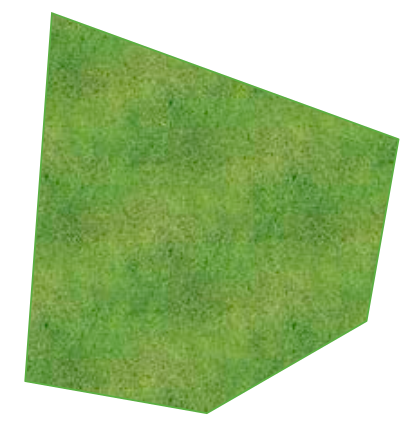
\includegraphics[width=.45\linewidth]{polygon2.png}
            \captionof{figure}{}
            \label{fig:polygon2}
          \end{figure}
        \end{minipage}

        \begin{enumerate}
          \item ¿Cuál es la longitud de la reja que Juan necesita para cercar su terreno?
          \item ¿Cuánta reja requiere Luis para cercar el suyo?
          \item Comparte tus procedimientos con un compañero. ¿Los consideran correctos? ¿Por qué?
        \end{enumerate}
  \item En parejas representen algebraicamente la longitud de uno de los lados y el perímetro de todo el terreno de Juan.
        \begin{enumerate}
          \item ¿Cuál de las longitudes del terreno de Luis será más adecuada para representar con la misma literal de tu
                respuesta anterior? ¿Por qué?
          \item Representen con una literal distinta la longitud mayor del terreno de Luis y expresen algebraicamente su
                perímetro.
          \item ¿Qué relación hay entre las longitudes de los lados distintos del terreno de Luis?
          \item A partir de su respuesta anterior, reescriban la expresión para el perímetro del terreno de Luis,
                pero usando una sola literal.
          \item ¿Cómo son entre sí las expresiones de los incisos b) y d)?
          \item ¿Qué cantidad de reja requieren Juan y Luis para rodear sus terrenos? Calculen a partir de las
                expresiones algebraicas que propusieron.
        \end{enumerate}

        \begin{boxH}
          Si dos variables están relacionadas, una de ellas se puede sustituir por la otra dentro
          de una expresión algebraica. Por ejemplo, si a es igual a $3b$, entonces la expresión
          $a + b$ es equivalente a $3b + b$, porque sustituimos a por $3b$.
          Un término algebraico en el que aparecen dos coeficientes se simplifica multiplicando
          los coeficientes, por ejemplo $3(4a)$ es equivalente a $12a$.
        \end{boxH}

        \subsubsection{El perímetro de un polígono regular}
        Una telaraña se forma por una sucesión de hexágonos regulares tales que la longitud de los
        lados de cada hexágono se incrementa en la misma cantidad con respecto a los lados del
        hexágono anterior (figura \ref{fig:web}).
        \begin{figure}[H]
          \centering
          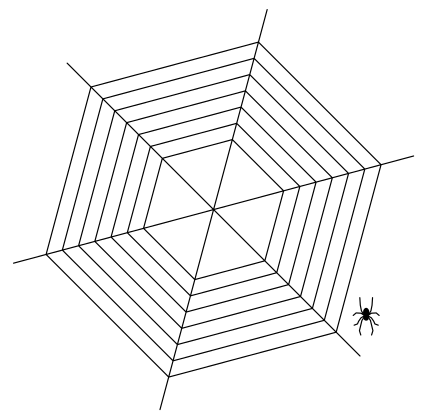
\includegraphics[width=.35\linewidth]{web.png}
          \captionof{figure}{}
          \label{fig:web}
        \end{figure}
        \begin{enumerate}
          \item En parejas escriban una expresión algebraica para representar
                el perímetro del hexágono más pequeño.
          \item Expresen algebraicamente la longitud de un lado del segundo
                hexágono a partir de la longitud de un lado del primero.
          \item Completen la tabla \ref{tab:tabla_web}.
                \begin{figure}[H]
                  \centering
                  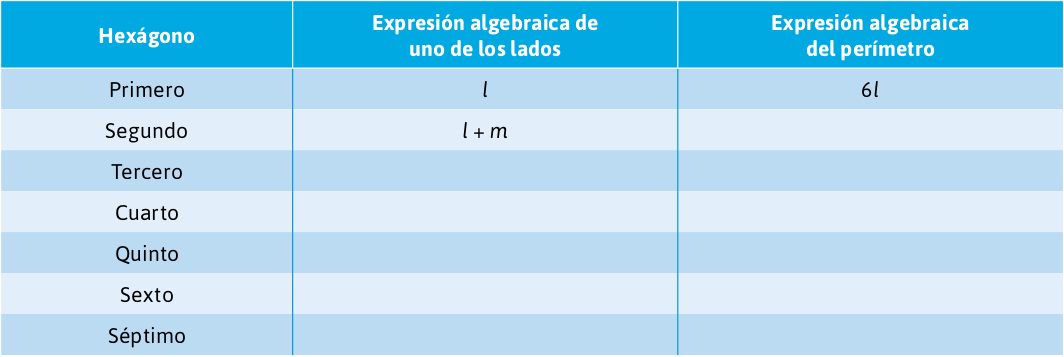
\includegraphics[width=.75\linewidth]{tabla_web.png}
                  \captionof{table}{}
                  \label{tab:tabla_web}
                \end{figure}
          \item Usa las expresiones anteriores para representar el total de hilo que ha segregado
                la araña. Simplifica los términos semejantes.
          \item Supón que el lado del hexágono menor mide 4.2 mm y el lado de cada hexágono
                subsecuente se incrementa en 8 mm, ¿cuáles son los perímetros de los diferentes
                hexágonos? Anótenlos en la tabla \ref{tab:tabla_lados}.
                \begin{figure}[H]
                  \centering
                  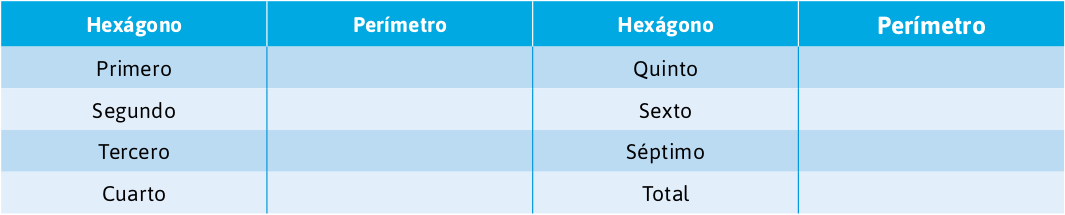
\includegraphics[width=.75\linewidth]{tabla_lados.png}
                  \captionof{table}{}
                  \label{tab:tabla_lados}
                \end{figure}
          \item Comparen en grupo sus respuestas y procedimientos. ¿Coincidieron los resultados?,
                ¿por qué? ¿Son iguales las expresiones algebraicas que propusieron? ¿Ocurrió que
                las expresiones fueran distintas, pero los resultados iguales? Si fue así, justifiquen
                esa situación; si no, encuentren el error.
          \item ¿Qué cantidad de hilo usó la araña para formar los hexágonos?
        \end{enumerate}
  \item Completa la tabla \ref{tab:tabla_polygons}.
        \begin{figure}[H]
          \centering
          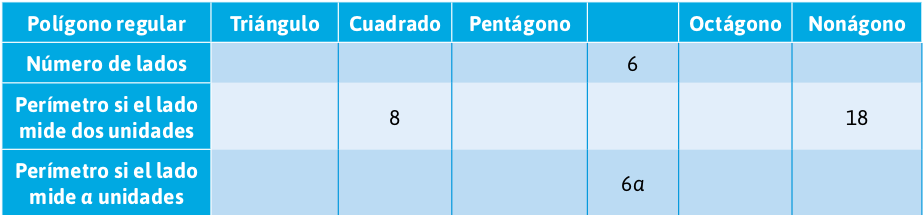
\includegraphics[width=.75\linewidth]{tabla_polygons.png}
          \captionof{table}{}
          \label{tab:tabla_polygons}
        \end{figure}
        \begin{enumerate}
          \item Determina una expresión algebraica para el perímetro de un polígono regular de $n$ lados.
        \end{enumerate}

        \begin{boxH}
          El perímetro de un polígono regular se calcula multiplicando la longitud de un
          lado por el número de lados de los que está compuesto.
        \end{boxH}

  \item Maribel compró una cuerda para forrar las cuatro caras laterales de una caja cúbica de 15 cm de lado.
        Con esa cuerda pudo rodear 30 veces la caja, pero le faltan
        por cubrir 5 cm a lo alto. Observa la figura \ref{fig:boxes}.

        \begin{minipage}{0.25\textwidth}
          \begin{figure}[H]
            \centering
            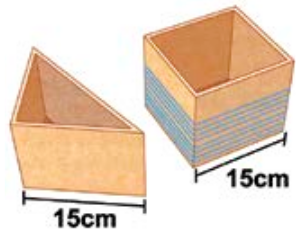
\includegraphics[width=\linewidth]{boxes.png}
            \captionof{figure}{}
            \label{fig:boxes}
          \end{figure}
        \end{minipage}\hfill
        \begin{minipage}{0.65\textwidth}
          \begin{enumerate}
            \item Maribel tiene otra caja con forma de prisma triangular que también mide
                  15 cm de lado. En equipos respondan: ¿en este caso sí le alcanzará la
                  cuerda para cubrir por completo la caja? Expliquen.
            \item ¿Cuál es el perímetro de la cara inferior de la caja cúbica?
            \item ¿Cuál es la longitud de la cuerda?
            \item ¿Cuál es el perímetro de la cara inferior de la caja con forma de prisma triangular?
            \item ¿Cuál es el perímetro de la cara inferior de la caja con forma de prisma triangular?
            \item A partir de sus respuestas a los incisos b), c) y d) escriban una justificación o corrijan
                  sus respuestas al inciso a).
          \end{enumerate}
        \end{minipage}

  \item Observa en la figura \ref{fig:hexagon} que los lados del hexágono regular grande miden el triple
        que los lados del hexágono regular pequeño. ¿Cuántas veces es más grande el perímetro del
        hexágono mayor respecto al del hexágono pequeño?

        \begin{minipage}{0.25\textwidth}
          \begin{figure}[H]
            \centering
            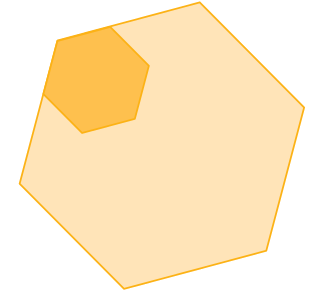
\includegraphics[width=\linewidth]{hexagon.png}
            \captionof{figure}{}
            \label{fig:hexagon}
          \end{figure}
        \end{minipage}\hfill
        \begin{minipage}{0.65\textwidth}
          \begin{enumerate}
            \item Escribe una expresión algebraica para el perímetro del hexágono pequeño a partir de la longitud de uno de sus lados.
            \item Expresa en términos de la longitud de los lados del hexágono pequeño la longitud de un lado del hexágono grande.
            \item Expresa algebraicamente el perímetro del polígono grande en términos de la longitud del hexágono pequeño.
            \item Compara tus respuestas y valídenlas con el grupo.
          \end{enumerate}
        \end{minipage}

  \item  Cinco amigos colocan sus toallas de baño sobre la playa formando un gran cuadrado como el de la figura \ref{fig:toallas}.
        Las toallas de Alicia y Beatriz son cuadradas, cada
        una de 720 cm de perímetro, mientras que las de Carlos, Diana y Emilio son rectangulares e iguales.
        \begin{minipage}{0.25\textwidth}
          \begin{figure}[H]
            \centering
            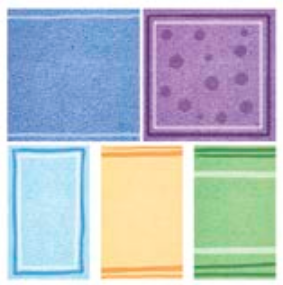
\includegraphics[width=\linewidth]{toallas.png}
            \captionof{figure}{}
            \label{fig:toallas}
          \end{figure}
        \end{minipage}\hfill
        \begin{minipage}{0.65\textwidth}
          \begin{enumerate}
            \item En equipos escriban una expresión algebraica que represente el perímetro de una de las toallas cuadradas si desconocen la longitud de sus lados.
            \item ¿Cuál es la longitud de los lados de las toallas de Alicia y Beatriz? Expliquen su procedimiento para obtener la respuesta.
            \item Escriban una expresión con las literales de la expresión algebraica del inciso a que represente el perímetro de las toallas rectangulares.
            \item Calculen las dimensiones de las toallas rectangulares. Expliquen su procedimiento.
          \end{enumerate}
        \end{minipage}

\end{enumerate}

\begin{boxK}
  \begin{center}\textbf{Cierre}\end{center}

  \begin{enumerate}
    \item Regresa a la sección Inicio y considera que las dimensiones de un paquete son $l$ cm de largo, $a$ cm de ancho y $h$ cm de alto.
          \begin{enumerate}
            \item Escribe una expresión algebraica que represente el total
                  de cordón necesario para amarrar el empaque.
            \item Explica el efecto de incrementar cada una de las dimensiones de la caja en la cantidad de cordón necesario
                  para amarrarla.
          \end{enumerate}
    \item En la figura \ref{fig:cuadrados}, I, II, III y IV son cuadrados. Si el perímetro del cuadrado I es 16 cm y
          el del cuadrado II, 24 cm, ¿cuál es el perímetro del cuadrado IV?
          \begin{figure}[H]
            \centering
            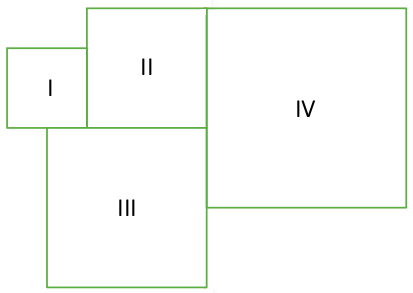
\includegraphics[width=.25\linewidth]{cuadrados.png}
            \captionof{figure}{}
            \label{fig:cuadrados}
          \end{figure}
    \item Dado un rectángulo con base $a$ y altura $b$, como el de la figura \ref{fig:rectangulo}
          escribe tres expresiones algebraicas que
          representen el perímetro de la figura \ref{fig:rectangulo}.
          \begin{figure}[H]
            \centering
            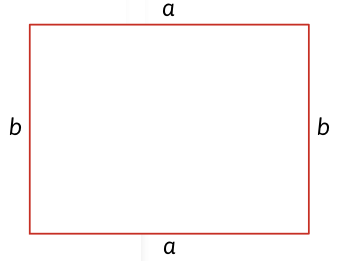
\includegraphics[width=.25\linewidth]{rectangulo.png}
            \captionof{figure}{}
            \label{fig:rectangulo}
          \end{figure}
    \item Dos hormigas van del punto A al punto B (figura \ref{fig:hormigas}).
          \begin{figure}[H]
            \centering
            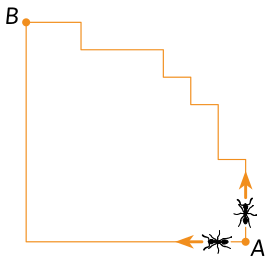
\includegraphics[width=.25\linewidth]{hormigas.png}
            \captionof{figure}{}
            \label{fig:hormigas}
          \end{figure}
          \begin{enumerate}
            \item ¿Qué hormiga recorre un trayecto más largo? Justifica su respuesta.
          \end{enumerate}
  \end{enumerate}
\end{boxK}


\subsection{Perímetro del círculo}

\begin{boxK}
  \begin{center}\textbf{Inicio}\end{center}

  \begin{enumerate}
    \item Ciro tiene un pequeño balón de basquetbol y necesita un aro de alambrón para encestarlo.
          Su balón mide 38 cm de circunferencia y un buen
          reto es encestarlo en un aro cuyo radio sea 5 cm más grande que el del
          balón.
          \begin{figure}[H]
            \centering
            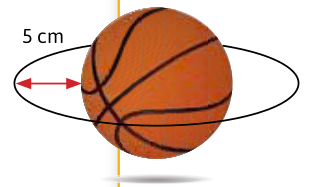
\includegraphics[width=.35\linewidth]{balon.png}
            \captionof{figure}{}
            \label{fig:balon}
          \end{figure}
          \begin{enumerate}
            \item ¿Qué cantidad de alambrón necesitará para elaborar su aro? Explica tu respuesta.
          \end{enumerate}
  \end{enumerate}
\end{boxK}

\begin{enumerate}
  \item Para medir el perímetro de figuras cuyo contorno está formado por segmentos
        rectos se puede usar una regla rígida. Cuando el contorno de una figura es
        curvo necesitamos recurrir a instrumentos flexibles, como las cintas métricas
        de los sastres.
        \begin{enumerate}
          \item En parejas midan el contorno de objetos circulares como los que se mencionan en
                la primera fila de la tabla. Escriban los datos correspondientes y realicen las
                operaciones para completar la tabla \ref{tab:tabla_rigidos}.\\

                \begin{figure}[H]
                  \centering
                  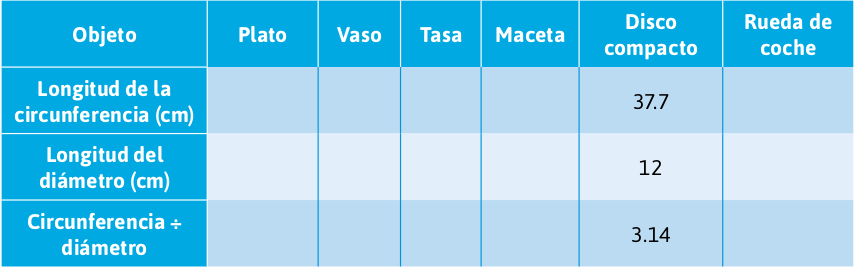
\includegraphics[width=.65\linewidth]{tabla_rigidos.png}
                  \captionof{table}{}
                  \label{tab:tabla_rigidos}
                \end{figure}

          \item Comparte en grupo los resultados de la última fila. ¿Qu\'e observas? Escribe una conclusión.
          \item En una calculadora científica oprime la tecla del símbolo $\pi$. ¿Qué valor se muestra? Anótenlo.
          \item Compara ese valor con los que obtuviste en la última fila de la tabla. ¿Qué observas?
                Escriban una conclusión entre todos.
        \end{enumerate}

        \begin{boxH}
          Desde la Antigüedad se sabe que en cualquier círculo hay una relación entre la longitud de la
          circunferencia y la longitud de su diámetro; a saber, la razón entre el perímetro del círculo y
          la longitud de su diámetro es constante.
          Este valor se denota con la letra griega $\pi$ (pi) y es un número decimal infinito no periódico
          cuyas primeras cifras son 3.14159\dots
          Para calcular el perímetro de un círculo, es decir, la longitud de su circunferencia utilizamos
          la expresión $P =\pi d$, donde d es la longitud del diámetro. ¿Por qué esa expresión es correcta?
        \end{boxH}

  \item En la figura \ref{fig:polygons_inside} están inscritos en el círculo un cuadrado,
        un octágono regular y un polígono regular de 16 lados.

        \begin{minipage}{0.3\textwidth}
          \begin{figure}[H]
            \centering
            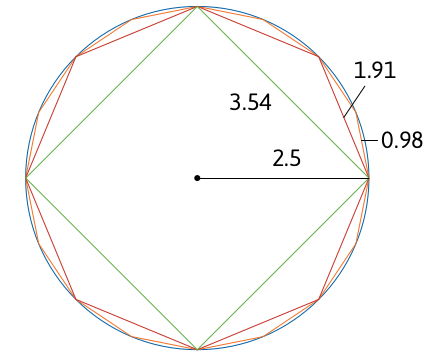
\includegraphics[width=\linewidth]{polygons_inside.png}
            \captionof{figure}{}
            \label{fig:polygons_inside}
          \end{figure}
        \end{minipage}\hfill
        \begin{minipage}{0.7\textwidth}
          \begin{enumerate}
            \item Calcula el perímetro de cada uno.
            \item Calcula el perímetro del círculo.
            \item Compara el perímetro de los polígonos con el perímetro del círculo. ¿Qué observas?
            \item Imagina un polígono regular de 32 lados inscrito en el círculo. ¿Cuál consideras
                  que será el valor aproximado de su perímetro? Justifica tu respuesta y compártela con el grupo.
          \end{enumerate}
        \end{minipage}

        \begin{boxH}
          Medir círculos con precisión es difícil, por eso desde la Antigüedad se propusieron
          métodos para calcular el perímetro de un círculo. Por ejemplo, Arquímedes, usando
          polígonos regulares \textbf{\color{cyan}inscritos y circunscritos} en una circunferencia, obtuvo una muy
          buena aproximación al número $\pi$. Demostró que su valor era un número entre $\frac{223}{71}$ y $\frac{21}{7}$.
          ¿Crees que esa aproximación sea correcta?
        \end{boxH}

        \begin{boxE}
          Polígonos \textbf{\color{cyan}inscritos y cirncunscritos}. Se dice que una figura esta inscrita en otra si cada
          uno de los vértices de la primera figura esta sobre el lado respectivo de la segunda figura.
          En esta misma situación se dice que la segunda figura esta circunscrita en la primera.
        \end{boxE}

        \begin{minipage}[t]{0.7\textwidth}
          \item En una casa de moneda necesitan estuches circulares de
          plástico para guardar centenarios, una moneda de oro mexicana cuya circunferencia es de 11.62 cm (figura \ref{fig:moneda}). ¿Cuál
          es el radio interior mínimo que deben tener un estuche para guardar este tipo de monedas?
        \end{minipage}\hfill
        \begin{minipage}[t]{0.2\textwidth}
          \begin{figure}[H]
            \centering
            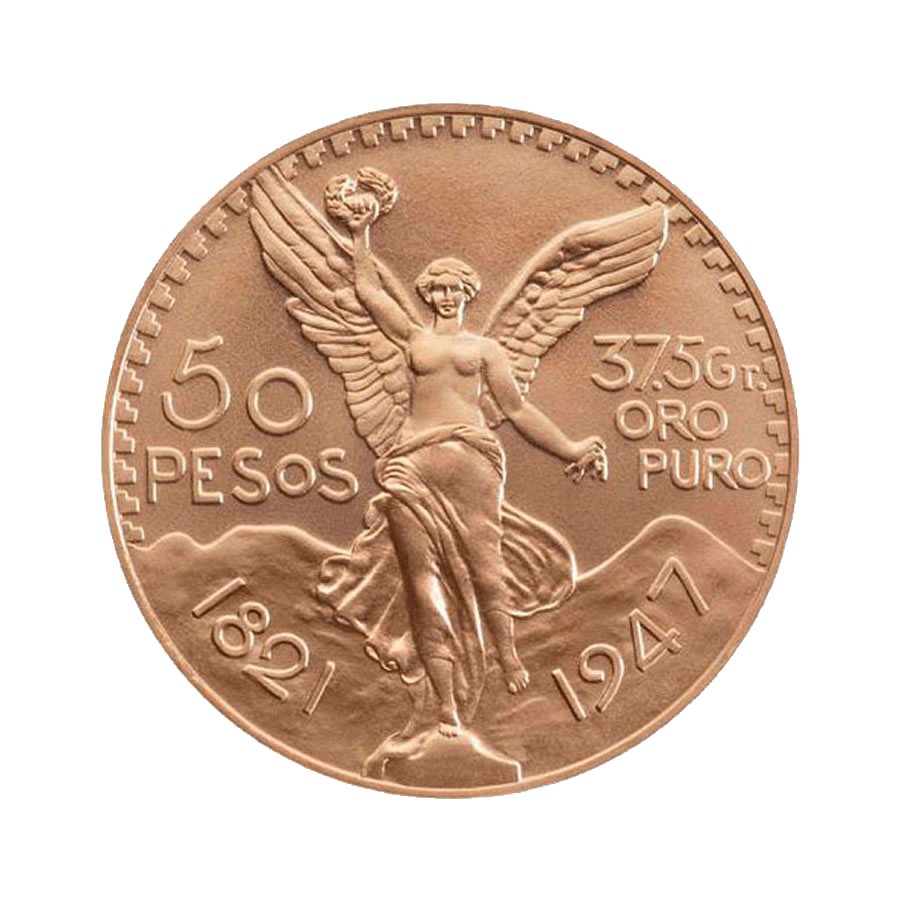
\includegraphics[width=\linewidth]{moneda.png}
            \captionof{figure}{}
            \label{fig:moneda}
          \end{figure}
        \end{minipage}



        \begin{minipage}[t]{0.7\textwidth}
          \item Una pista de atletismo debe tener dos partes rectas y dos partes formadas por
          semicírculos. Cada una de las rectas debe medir 100 m de largo, y la longitud de
          cada semicírculo también debe ser de 100 m (figura \ref{fig:pista}). ¿Cuánto mide el radio de los semicírculos?
        \end{minipage}\hfill
        \begin{minipage}[t]{0.2\textwidth}
          \begin{figure}[H]
            \centering
            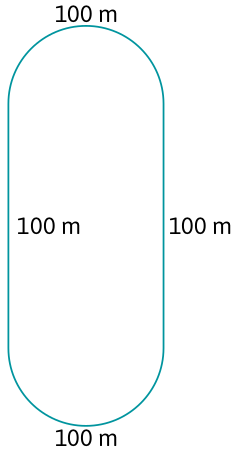
\includegraphics[width=\linewidth]{pista.png}
            \captionof{figure}{}
            \label{fig:pista}
          \end{figure}
        \end{minipage}

        \begin{minipage}[t]{0.2\textwidth}
          \begin{figure}[H]
            \centering
            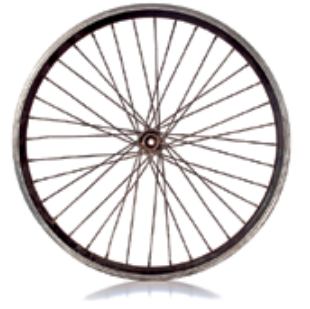
\includegraphics[width=\linewidth]{rueda.png}
            \captionof{figure}{}
            \label{fig:rueda}
          \end{figure}
        \end{minipage}\hfill
        \begin{minipage}[t]{0.7\textwidth}
          \item Una rueda de bicicleta está formada por un buje central donde se enganchan los
          rayos. El otro extremo de los rayos se sujetan a un aro metálico donde se coloca
          la llanta (figura \ref{fig:rueda}). Considera que el diámetro de la llanta es de 71.12 cm.

          \begin{enumerate}
            \item ¿Qué distancia recorre la bicicleta cuando la llanta da una vuelta completa?\\
            \item ¿Qué distancia recorre si las llantas dan diez vueltas completas?\\
            \item ¿Cuántas vueltas deben dar las llantas para recorrer un kilómetro?\\
            \item Los odómetros de los automóviles son instrumentos que miden la distancia que éste
                  recorre y normalmente están conectados a mecanismos de las llantas. Explica su funcionamiento.
          \end{enumerate}
        \end{minipage}

        \begin{minipage}[t]{0.7\textwidth}
          \item Sofía hace un diseño con círculos y semicírculos, como en la figura \ref{fig:jinjang}, y piensa
          cubrir las líneas del círculo y de los semicírculos con cordón dorado.
          \begin{enumerate}
            \item ¿Cuánto cordón necesitará para cubrir la circunferencia más grande?\\
            \item ¿Y para cubrir los dos semicírculos interiores?\\
            \item ¿Qué relación hay entre la longitud del círculo y las de los semicírculos? Explica tu respuesta.
          \end{enumerate}
        \end{minipage}\hfill
        \begin{minipage}[t]{0.2\textwidth}
          \begin{figure}[H]
            \centering
            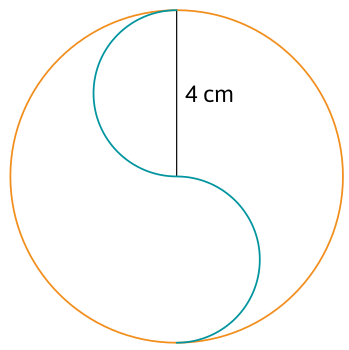
\includegraphics[width=\linewidth]{jinjang.png}
            \captionof{figure}{}
            \label{fig:jinjang}
          \end{figure}
        \end{minipage}


  \item Un autódromo tiene la forma y las dimensiones que ilustra la figura \ref{fig:autodromo}.
        \begin{figure}[H]
          \centering
          \includegraphics[width=.8\linewidth]{autodromo.png}
          \captionof{figure}{}
          \label{fig:autodromo}
        \end{figure}
        \begin{enumerate}
          \item Calcula la distancia que cubre un auto al recorrer una vez el circuito por el carril interno.\\
          \item Calcula la distancia que se recorre en un auto al conducir una vez por el carril externo.\\
          \item A qué distancia se deben separar dos autos en una carrera de una vuelta para que ambos recorran la misma distancia.
        \end{enumerate}
  \item Carlos mandó construir una ventana con la forma y las medidas que aparecen en
        la figura \ref{fig:ventana}. ¿Qué longitud de material fue necesario para formar el contorno de la ventana?

        \begin{figure}[H]
          \centering
          \includegraphics[width=.3\linewidth]{ventana.png}
          \captionof{figure}{}
          \label{fig:ventana}
        \end{figure}
        \newpage
  \item Se construyó una cancha de basquetbol (figura \ref{fig:cancha}) y se quieren pintar todas sus
        líneas: círculo central, área de foul, línea de tres puntos, etcétera. Calcula la longitud de todas las líneas que se deben pintar.
        \begin{figure}[H]
          \centering
          \includegraphics[width=.8\linewidth]{cancha.png}
          \captionof{figure}{}
          \label{fig:cancha}
        \end{figure}

  \item En equipos compartan y validen sus respuestas a los ejercicios del 3 al 9. Organícense
        para que cada equipo exponga la solución de un ejercicio al resto del grupo.
\end{enumerate}

\begin{boxK}
  \begin{center}\textbf{Cierre}\end{center}
  \begin{enumerate}
    \item Regresa a la situación de Inicio y determina el diámetro del balón de Ciro.
          \begin{enumerate}
            \item ¿Cuánto debe medir el diámetro del aro?
            \item ¿Qué tanto alambrón necesita Ciro para el aro?
          \end{enumerate}
    \item Un avión supersónico dará una vuelta alrededor de la Tierra sobre el
          ecuador a una altura promedio de 10,000 m. Considera que la circunferencia de la Tierra es de 40,066.4 km.
          \begin{enumerate}
            \item ¿Qué distancia habrá recorrido el avión al cumplir su objetivo?
          \end{enumerate}
    \item Las ciudades de Chicago y Estambul están sobre un mismo paralelo de
          nuestro planeta. Si el radio de la circunferencia que constituye ese
          paralelo es de 4,000 km:
          \begin{enumerate}
            \item ¿Qué distancia se debe recorrer sobre la superficie de la Tierra para
                  ir de una ciudad a otra sobre ese paralelo? Considera que los radios
                  del centro de la Tierra hacia las ciudades forman un ángulo de 120°,
                  esto es, la distancia entre ellas es la tercera parte del paralelo.
          \end{enumerate}
    \item Comparte y valida tus respuestas con el resto de tus compañeros.
  \end{enumerate}
\end{boxK}

\newpage
\subsection{Áreas de triángulos y cuadriláteros}

\begin{boxK}
  \begin{center}\textbf{Inicio}\end{center}

  \begin{enumerate}
    \item Un arquitecto diseña dos escuelas que se construirán en terrenos como las figuras \ref{fig:arqui}.
          \begin{figure}[H]
            \centering
            \includegraphics[width=.5\linewidth]{arqui.png}
            \captionof{figure}{}
            \label{fig:arqui}
          \end{figure}
          \begin{enumerate}
            \item Observa ambas figuras. ¿Qué terreno consideras que tiene mayor área? ¿Por qué?
            \item Realiza las mediciones necesarias y verifica tu respuesta.
            \item ¿Cómo calculaste el área de las figuras? Explica tu respuesta.
          \end{enumerate}
  \end{enumerate}
\end{boxK}















\newpage \thispagestyle{plain}
\section{Ecuaciones lineales}

\boxabstract{Aprendizajes esperados}{Resuelve problemas mediante la formulación y solución algebraica de ecuaciones lineales.}

\subsection{Formulación de ecuaciones}

\subsection{Solución de una ecuación}




\newpage \thispagestyle{plain}
\section{Resolución de ecuaciones lineales}

\boxabstract{Aprendizajes esperados}{Resuelve problemas mediante la formulación y solución algebraica de ecuaciones lineales.}


\subsection{Propiedades de la igualdad}


\subsection{Más sobre ecuaciones lineales}






\newpage \thispagestyle{plain}

\section{Medidas de tendencia central}

\boxabstract{Aprendizajes esperados}{Aprendizajes esperados}{Usa e interpreta las medidas de tendencia central (moda, media aritmética y mediana) y el
  rango de un conjunto de datos, y decide cuál de ellas conviene más en el análisis de los datos en cuestión.}

\subsection{Media aritm\'etica o promedio}

\subsection{La media aritmética y el rango}





\newpage \thispagestyle{plain}
\section{Moda, media aritmética y mediana}

\boxabstract{Aprendizajes esperados}{Aprendizajes esperados}{Usa e interpreta las medidas de tendencia central (moda, media aritmética y mediana) y
  el rango de un conjunto de datos, y decide cuál de ellas conviene más en el análisis de los datos en cuestión.
}

\subsection{Media aritm\'etica y mediana}

\subsection{Moda}
\subsection{Representantes de un grupo de datos}

\chapter{}

\section{Situaciones de variación proporcional}

\subsection{Comparación de situaciones de variación proporcional con tablas}

\subsection{Comparación de situaciones de variación proporcional con gráficas}

\subsection{Comparación de situaciones de variación proporcional con expresiones algebraicas}




\newpage \thispagestyle{plain}

\section{Pendiente de una recta y razón de cambio}

\subsection{Variación proporcional y pendiente}

\subsection{Razón de cambio y variación}

\subsection{Efectos en la recta al cambiar la pendiente}

\newpage \thispagestyle{plain}

\section{Análisis y comparación de situaciones de variación lineal}

\subsection{Efectos de la recta al cambiar la ordenada al origen}

\subsection{Situaciones de variación lineal asociadas a la física, la biología y la economía}

\newpage \thispagestyle{plain}

\section{Sucesiones y expresiones algebraicas}

\subsection{Sucesiones numéricas}

\subsection{Sucesiones con progresión aritmética}


\newpage \thispagestyle{plain}

\section{Congruencia de triángulos y aplicaciones}

\subsection{Aplicaciones de congruencia de triángulos}

\subsection{Aplicaciones a cuadriláteros}

\newpage \thispagestyle{plain}

\section{Vol\'umenes de prismas rectos}

\subsection{Volumen de prismas rectos rectangulares}

\subsection{Fórmula del volumen de prismas rectos}


\newpage \thispagestyle{plain}

\section{Gráficas circulares}

\subsection{Recolecta y registra datos}

\subsection{Registra datos en gráficas circulares}

\subsection{Leer e interpretar datos en gráficas circulares}

\newpage \thispagestyle{plain}

\section{El azar y la probabilidad frecuencial}

\subsection{Tipos, recolección y organización de datos}

\subsection{Experimentos aleatorios y deterministas}

\subsection{Espacio muestral de un experimento aleatorio}

\subsection{Cálculo de la probabilidad frecuencial}


\end{document}





